\section{Unstructured \p\ Networks}
\label{section:unstructured}

In this section, we present algorithms that tackle the topology mismatch
problem in unstructured \p\ networks and classify them based on their 
use of the overlay structure, their message forwarding scheme 
for peer communication as well as techniques used for detecting proximity 
in order to optimize their overlay topology.

% TODO: READ A Near-Optimal Algorithm Attacking the Topology Mismatch Problem in
%Unstructured Peer-to-Peer Networks (This is an Approximation alg for Top-mis
%problem)

%%%%%%%%%%%%%%%%%%%%%%%%%%%%%%%%%%%%%%%%%%%%%%%%%%%%%%%%%%%%%%%%%%%%%%%%%%%%%%%%
%
% TODO: HOW CAN UNSTRUCTURED SCHEMES BE REFINED
%
%For this reasons, efforts have been placed for optimizing the efficiency of
%decentralized unstructured peer-to-peer networks. Research mainly focuses on
%\begin{inparaenum}[\itshape i\upshape)]
%  \item reducing unnecessary, redundant communication traffic, and
%  \item exploiting physical locality to reduce communication response.
%\end{inparaenum}
%The goal can be achieved at, both, the application-level network as well as the
%underlying physical one. In the first case by refining the message relay
%techniques, while in the second one, by adaptively reconstructing the
%application network to map as well as possible to the the physical network.
%
%%%%%%%%%%%%%%%%%%%%%%%%%%%%%%%%%%%%%%%%%%%%%%%%%%%%%%%%%%%%%%%%%%%%%%%%%%%%%%%%


\subsection{Algorithms for Unstructured Architectures}

% BROADCAST OPTIMIZATION

%%%%%%%%%%%%%%%%%%%%%%%%%%%%%%%%%%%%%%%%%%%%%%%%%%%%%%%%%%%%%%%%%%%%%%%%%%%%%%%%
% \subsubsection{Improving search in peer-to-peer networks}

% \begin{figure}[ht]
% \centering
% \subfigure[Iterative deepening with three levels.] {
%   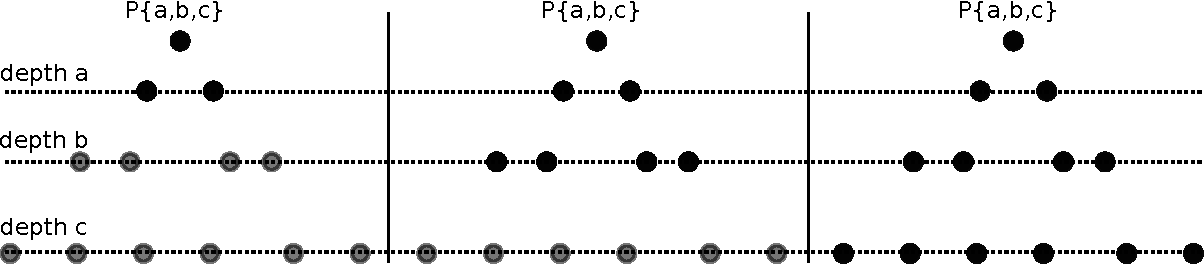
\includegraphics[scale=0.4]{img/algorithms/iterative_deepening}
%   \label{figure:dbfs:iterdeep}
% }\qquad\qquad
% \subfigure[Directed BFS.] {
%   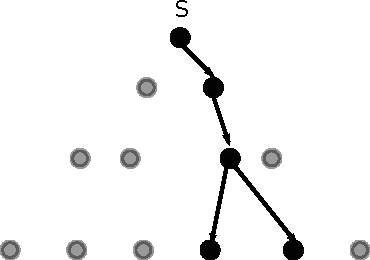
\includegraphics[scale=0.4]{img/algorithms/directed_bfs}
%   \label{figure:dbfs:dbfs}
% }\qquad\qquad
% \subfigure[Local indices with radius size equal to $2$.] {
%   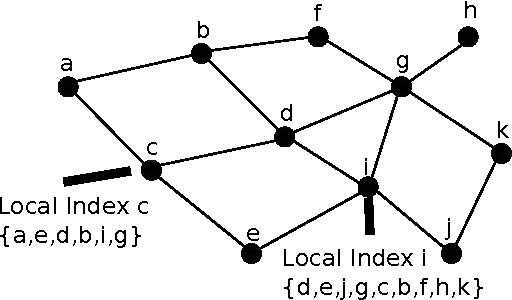
\includegraphics[scale=0.4]{img/algorithms/local_indices}
%   \label{figure:dbfs:localindx}
% }
% \caption{Improving search in P2P networks}
% \label{figure:dbfs}
% \end{figure}

To improve over {\sl Gnutella}'s ``blind flooding'' approach,
\cite{YG-M2002} proposed a practical and easy to implement solution 
weaved around three different message forwarding methods:
\emph{iterative deepening},
\emph{directed BFS}, and \emph{local indices}.
%%AD local indices is not "a message forwarding method" really...  but ok.

In \emph{iterative deepening}, 
%(see Figure~\ref{figure:dbfs:iterdeep})
the search is
performed on a BFS tree with multiple preset depths. 
The depth limit is iteratively increased by the source node for each query, 
based on the quality of the results. 
The source node may issue a new request with increased depth limit
that will trigger the nodes at the last depth level to resume the search. 
The iterative approach avoids restarting the entire search process 
from scratch at each iteration and reduces the load on the nodes of 
the upper levels of the tree. 
Its major drawback is the delay between successive iterations, as the
source-node has to examine the results at each iteration before deciding to
either quit or resume the query.

The \emph{directed BFS}
tries to avoid the aforementioned delay by forwarding 
the query messages only to a select set of neighbors, in which the selection criteria varies from the number of
results received previously, distance in terms of hops, bandwidth, or the query
load of the neighbor.
%
In \emph{local indices},
each node indexes data within a radius of $r$ hops and uses 
this local index to answer queries % on behalf of them 
without generating additional traffic. Local indices
greatly reduce the aggregate bandwidth usage of the network and 
improve query efficiency. However, updating such indices in 
the presence of frequent node joins/departures 
may introduces significant overhead should the radius is kept broad.
Below, we outline how the techniques in~\cite{YG-M2002}
fare against the $3$ major performance criteria 
of Section~\ref{section:background}.
% \begin{center}
% \begin{tabular}{ccc}
% \textbf{Efficiency} & \textbf{Overhead} & \textbf{Scalability} \\
% \hline
% Iterative Deepening & ? & ? & ?
% Directed BFS & ? & ? & ?
% Local Indices & ? & ? & ?
% \end{tabular}
% \end{center}
\begin{center}
{\footnotesize
\begin{tabular}{rccc}
\multicolumn{1}{r}{} &
\multicolumn{1}{c}{\emph{Efficiency}} &
\multicolumn{1}{c}{\emph{Overhead}} &
\multicolumn{1}{c}{\emph{Scalability}}
\\
\cline{2-4}
\emph{Iterative Deepening} &
% needs recalculation in every iteration step
% extra delay imposed in a high churn environment that prohibits the algorithm
% to start from the last level of nodes and results in a restart of the whole
% process
low &
% the process in not started from the beginning at each iteration step
low &
% 
medium \\
\emph{Directed BFS} &
% Better time to satisfaction compared to iterative deepening
medium &
% Better quality and quicker results mean more aggregate bandwidth and
% processing power needs to be consumed since more nodes are involved (death
% spiral).
medium &
% BFS is Gnutella's non efficient communication method
medium \\
\emph{Local Indices} &
% efficiency is enhanced greatly since data pointers are replicated across the
% network
high &
% updating indices is a time and resource consuming process.
medium &
% the scalability is constrained by the indices update in a highly dynamic
% environment (high churn)
medium \\
\end{tabular}
}
\end{center}

%%%%%%%%%%%%%%%%%%%%%%%%%%%%%%%%%%%%%%%%%%%%%%%%%%%%%%%%%%%%%%%%%%%%%%%%%%%%%%%%
% \paragraph*{ \bf Delay Aware P2P System}
% A new \emph{Delay Aware P2P System (DAPS)} is introduced in \cite{ZL2005}. 
A \emph{delay--aware} \p\ system termed {\sl DAPS} 
was introduced in~\cite{ZL2005}.
{\sl DAPS}  seeks to attain reduced look-up times by dividing 
peer routing tables into several sectors of increasing delay. 
The source node that issues the query designates the delay 
boundary it may tolerate providing so a \emph{pruning factor}.
In this context, user requests are forwarded only to 
nodes whose expected delay is less than or equal to the indicated boundary. 
{\sl DAPS} primarily focuses on user ``experience'' and deploys a
end-to-end delay monitoring mechanism that  may enable
the clustering of routing tables. 
In an dynamic environment, the formation 
of very accurate such routing tables might be however an elusive goal.
%With the clustered
%routing tables and the loose organization of DAPS' overlay network it is
%considered by is be tween structured and unstructured.
%%
% TODO: MAYBE REVIEW THE EVALUATION
In terms of the $3$ performance criteria, {\sl DAPS} stands as follows:
\begin{center}
{\footnotesize
\begin{tabular}{ccc}
\emph{Efficiency} & \emph{Overhead} & \emph{Scalability} \\
\hline
%
low &
%
low &
%
medium
\end{tabular}
}
\end{center}

%%%%%%%%%%%%%%%%%%%%%%%%%%%%%%%%%%%%%%%%%%%%%%%%%%%%%%%%%%%%%%%%%%%%%%%%%%%%%%%%
% \subsubsection{Gia}

The key objective of the {\sl Gia} system~\cite{CRBLS2003} is 
to help alleviate the scalability omnipresent
in unstructured \p\ file-sharing systems.
At first, {\sl Gia} replaced {\sl Gnutella}'s blind flooding 
with random walks.
Although this adoption was 
a step in the right direction~\cite{lv_randomwalks_2002},
issuing a single copy of the query within the network
effectively reduces the search scope and may negatively affect 
the success rate of the query in question.
To overcome this limitation, {\sl Gia} introduces
a token-based flow control mechanism
% , which is essentially an intelligent flow control algorithm 
%%AD what is "intelligent"?? - I think you can live without this above line... 
that gradually redirects queries to nodes which are more
likely to answer. 
%%
This flow control mechanism also helps prevent node overloading
as each peer ``announces'' the number of query requests it 
can handle in terms of tokens to its neighbors; to this end, 
peers only forward query requests to nodes that they previously
received tokens from.
%%AD changed below as above... I have the impression that this token 
%%	based mechanism is one and the same (the way the writing appeared 
%%	was that they were two mechanisms!  check!!!
%%%%
% In order to prevent overloading of nodes with query requests,
% Gia uses a token-based flow control algorithm in which each node announces the
% number of query requests it can handle in terms of tokens to its neighbors, so
% that neighbors only forward query requests to nodes that they previously
% received tokens from. 
%%%%%%%%%%%%%%%%%
{\sl Gia} also acknowledges the heterogeneity in peer bandwidth,
processing power, disk speed, etc., of \p\ nodes and uses this
information when connecting nodes to each other.
By using a topology adaptation algorithm, 
{\sl Gia} places low capacity nodes within 
short proximity to peers with high performance features.
This topology adaptation algorithm is based on the metric 
each node maintains about its satisfaction --ranging between $0$ and $1$--
for the neighbors it finds itself associated with. 
Through message exchange, a peer can establish new connections 
or drop superseded one in order to improve its satisfaction.
%%AD the 2 lines below make no sense.. I rephrased as above... 
% \emph{Gia} ensures that high capacity nodes have high degrees and
% low capacity nodes are within short proximity to high capacity ones.
%%%%%%%%AD this (above) phrase is almost verbatim out of the paper! NO good idea ;-)
Despite the fact that {\sl Gia}'s topology adaptation algorithm 
that primarily focuses on the satisfaction of peers improves the network's 
scalability, it falls short in addressing the mismatch problem
as considerations for the underlying network are not handled in explicit
terms.
%%AD the comment TODO is somewhat correct. Changed the wording here..... 
% TODO: THIS FOLLOWING REMARK SOUNDS LIKE THE ALGORITHM SHOULDN'T BE IN THIS
%       SURVEY AFTER ALL!!
% Although the topology adaptation algorithm Gia uses improves the scalability of
% the network, it does not help much in solving the topology mismatch problem,
% since it does not consider the underlying physical topology.
%
%More specifically, there are four key components in the design of
%\emph{Gia} which are summarized bellow:
%\begin{enumerate}
%  \item A \emph{dynamic topology adaptation} protocol that puts
%participating nodes within short reach of high capacity nodes so that these
%\emph{high-degree} nodes, which due to their high connectivity receive most of
%the queries, actually have the capacity to handle them.
%  \item An \emph{active flow control} scheme is used to avoid overloaded
% hot-spots. Heterogeneity is detected and flow control tokens are given to
%nodes based on the available capacity.
%  \item Every node maintains pointers to to the content that is offered by
% their immediate neighbors, creating a \emph{one-hop replication} of pointers,
%scheme.
%  \item A \emph{search protocol} based on random walks, that is biased towards
% directing queries to high-capacity nodes that are typically best able to
%answer these queries.
%\end{enumerate}
%
In terms of the $3$ stated criteria, {\sl Gia}'s approach is as follows:
%%
%%AD from the discussion I think that Efficiency might me medium-how??? 
\begin{center}
{\footnotesize
\begin{tabular}{ccc}
\emph{Efficiency} & \emph{Overhead} & \emph{Scalability} \\
\hline
% Drastically reduces the search scope.
low &
% Only one copy of the query is issued to the network.
% A token based flow control mechanism redirects queries to nodes that are most
% likely to fulfill them.
low &
% Even thought the low overhead scalability is reduced by the reducing of
% search scope.
medium
\end{tabular}
}
\end{center}

% \begin{center}
% \begin{tikzpicture}
% \begin{axis}[
%   ybar,
%    symbolic x coords={
%      Efficiency,
%      Overhead,
%      Scalability
%    },
%    symbolic y coords={lo, med, hi},
%    x tick label style={rotate=45,anchor=east},
%    xtick=data, ytick=data
% ]

% \addplot coordinates {
%   (Efficiency,lo)
%   (Overhead,lo)
%   (Scalability,lo)
% };

% \end{axis}
% \end{tikzpicture}
% \end{center}



%%%%%%%%%%%%%%%%%%%%%%%%%%%%%%%%%%%%%%%%%%%%%%%%%%%%%%%%%%%%%%%%%%%%%%%%%%%%%%%%
% \subsubsection{Distributed Cycle Minimization Protocol (DCMP)}
% We have already discussed that blind flooding often causes messages 
% to be routed in a direction
% that is far from the path that can
% ultimately fulfill the query request. 
%%AD the above is just repetition... 

Another problem with topology unaware
systems is the duplication of messages due to cycles that appears 
 even along the correct forwarding path. 
\cite{ZKB2008}~focuses on this exact deficiency
of overlay networks and introduces the \emph{Distributed Cycle Minimization Protocol
(DCMP)}, a dynamic, fully distributed method that removes cycles;
this is accomplished without sacrificing
overlay connectivity, resilience and other key properties of unstructured
\p\ architectures and by avoiding a hierarchical organization of peers. 
Once a cycle is detected in {\it DCMP}, the most powerful node in that cycle 
is elected as the \emph{Gate Peer} and the cycle is then broken 
%% at a strategic place  %%AD I am not sure what this adds?? strategic?? on what??
so that it results in the minimization of the distance between the 
\emph{Gate Peer} and all other nodes that are currently part of the cycle. 
This process is managed by using two specialized message types 
namely, \emph{Information Collection (IC)} and \emph{Cut Message (CM)}. 
\emph{DCMP} bases its operation on messages whose travel is limited by 
imposed $TTL$ whose maximum value is set at  $7$ for most cases. 
This inherently limits the protocol as \emph{DCMP} is unlikely that 
can efficiently detect cycles that span for more than $7$ nodes.
%%AD rephrased as above
% One disadvantage of DCMP is that since the distance a forwarded
% message can travel is limited by the TTL value, which is practically $7$ in most
% cases, DCMP cannot detect cycles formed by more than 7 peers. 
Even though cycle elimination does improve network performance, 
it cannot 
% actually solve 
directly contribute in the solution of 
the topology mismatch problem.
%%
%
%\subsection{Distributed Cycle Minimization Protocol}
%
%\paragraph{}
%The first step after detecting a duplicate message by some peer is to gather
% information from all peers in the cycle using a new type of control message
%called \emph{Information Collecting Message} or \emph{ICM}. ICM contains:
%\begin{inparaenum}[\itshape i\upshape)]
%  \item a \emph{GUID}\footnote{Globally Unique Identifier assigned to every
% query message generated by any node.} field same as the one of the duplicate
%message,
%  \item \emph{DetectionID} field which represents the direction of the
% connection where the duplicate was identified\footnote{This ensures the
%uniqueness of the ICM messages because as it travels through many cyclic paths,
%multiple peers will detect the duplicates and initiate an ICM message.}, and
%  \item \emph{Node Information Vector (NIV)} which contains information
% (bandwidth, CPU power, etc) about peers that propagated the ICM.
%\end{inparaenum}
%
%\paragraph{}
%Suppose $A$ detected the duplicate as depicted in Figure~\ref{figure:dcmp}. It
% then emits an ICM to $B$ and $F$, that initially contains information only
%about itself. Each peer that receives the ICM, appends its information and
%propagates it along the reverse path of the original message. Since two copies
%of ICM are sent, at some point, a peer, say peer $D$, will receive a duplicate
%ICM. Using the information in the NIVs of the ICMs, $D$, decides to cut (for
%example) the EF connection. To inform the other peers about its decision, it
%emits a \emph{Cut Message (CM)} which contains the GUID and DetectionID of the
%corresponding ICM and an additional field that identifies the connection to be
%cut. $D$, then, forwards the CM in the reverse directions from where the ICM
%arrived. Similarly CMs received by any peer are propagated toward the reverse
%path of the corresponding ICM. Eventually, either peer $E$ or peer $F$ will
%receive the CM and cut the connection, thus eliminating the cycle.
%
%Receiving a duplicate ICM denotes the existence of a cycle. The opposite is not
% true though. For example, if the cycle contains $2 \times TTL$ edges, it will
%not be detected, because the ICM messages will be discarded before they locate
%it. There is a trade-off between preserving the connectivity of the network and
%minimizing the duplicates that makes such a possibility to be safely ignored.
%
%\begin{figure}
%\centering
%  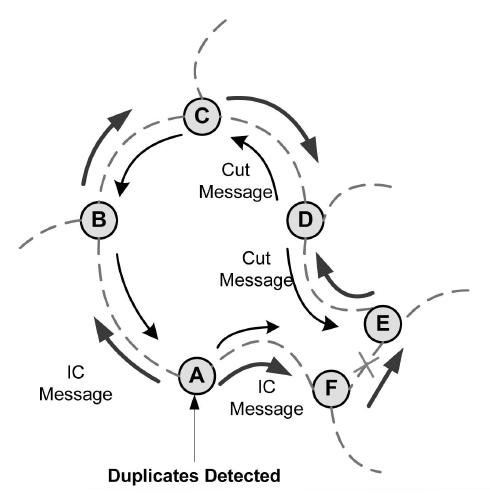
\includegraphics[scale=0.4]{img/dcmp.jpeg}
%\caption{Cycle elimination methods in DCMP}
%\label{figure:dcmp}
%\end{figure}
%
%\paragraph{}
%
% TODO: SOME DISCUSSION
%
%Actually, the duplicate packet problem seems to hurt more the active nodes;
%those with higher capacities and bandwidth that contribute the most to the
%network.
The expected \emph{DCMP} behavior as far as our $3$ criteria is:
%
\begin{center}
{\footnotesize
\begin{tabular}{ccc}
\emph{Efficiency} & \emph{Overhead} & \emph{Scalability} \\
\hline
% It return more result than LTM according to experiments in
% \cite{ZKB2008}
medium &
% Duplicates are an important fraction of the redundant overhead imposed by
% topology mismatch and thus DCMP minimizes this as possible.
% The control overhead is also one to two orders of magnitude less than LTM due
% to its ``lazy'' broadcasting of control messages (as opposed to LTM's periodic
% approach) - \cite{ZKB2008}
low &
% fully distributed method
high
\end{tabular}
}
\end{center}

%       CACHING

%%%%%%%%%%%%%%%%%%%%%%%%%%%%%%%%%%%%%%%%%%%%%%%%%%%%%%%%%%%%%%%%%%%%%%%%%%%%%%%%
% \subsubsection{Replication Strategies in Unstructured Peer-to-Peer Networks}

In~\cite{CS2002}, replication is used as a way 
to improve inefficient blind search.
As the number of replicas and/or cached copies increases in the network,
it would relatively easy to locate items even if the search is random.
% \cite{CS2002} aim to improve the inefficient blind search algorithm by
% replicating the data in a P2P network. 
% The main intuition behind the
% idea of replication, or using cached copies, is that as the number of copies for
% each item increases in the network, it would be easier for a search algorithm,
% even a random one, to locate these items. 
To analyze the feasibility of
such an approach, \cite{CS2002} investigates $3$ replication
strategies: uniform, proportional, and square-root allocation. In the
uniform model, the copies of items are uniformly spread over the network,
while in the proportional, items are replicated based on their query
rate, so that frequently queried items can be found more often. 
The square root is a compromise between uniform 
and proportional allocation models.
% allocation is a strategy proposed by Cohen and Shenker, which is a model between
% the uniform and proportional allocation.  
%%AD why u need to say the name here????
The overall costs for both successful and unsuccessful
searches are compared to ascertain the effectiveness of the $3$ suggested 
approaches.
% To evaluate the outcome of the replication models, 
% the overall costs of successful and unsuccessful
% searches in the network are compared. 
Experimental outcomes indicate that the uniform allocation 
minimizes the maximum search length and so it can 
reduce the time spent on unsuccessful searches.
% Results argue that the uniform allocation %%AD results argue???? --
					    %% ALSO, "search size??? See above
% model minimizes the maximum search size, therefore reduces the time spent on an
% unsuccessful search. 
The proportional strategy effectively decreases the search time 
for popular items, but suffers when needing to locate the rare entities.
% The proportional model, on the other hand, promotes the
% more frequently queried items by replicating them more and therefore decreases the
% search time for popular items, but suffers when needing to locate the rare
% items. 
When it comes to expected successful search size, it is the same for 
for both uniform and proportional models and any approach in between 
to always behave much better.
% The authors also claim that the expected successful search size is the
% same for uniform and proportional models, and any approach between them would
% always behave much better. 
The square root allocation  aims at minimizing the 
expected search size for successful queries in \p\ networks.
% Finally, they propose the square root allocation
% approach, which is a replication strategy that minimizes the expected search
% size of successful queries in P2P networks.
%%
The table below outlines how the $3$ strategies fare:
%%
\begin{center}
{\footnotesize
\begin{tabular}{rccc}
\multicolumn{1}{r}{} &
\multicolumn{1}{c}{\emph{Efficiency}} &
\multicolumn{1}{c}{\emph{Overhead}} &
\multicolumn{1}{c}{\emph{Scalability}}
\\
\cline{2-4}
\emph{Uniform Replication} &
% Proportional and Uniform are the worst “reasonable” strategies
low &
% When item is created, replicate its key in a fixed number of hosts.
low &
%
medium \\
\emph{Proportional Replication} &
% Proportional and Uniform are the worst “reasonable” strategies
low &
% for each query, replicate the key in a fixed number of hosts (need to know or
% estimate the query rate)
medium &
%
low \\
\emph{Square Root Replication Allocation} &
% All (strictly) in-between strategies are (strictly) better than Uniform and
% Proportional - replication theory
medium &
% Assuming that each query keeps track of the search size then each time a query
% is finished the object is copied to a number of sites proportional to the
% number of probes that the search required.
medium &
% e.g. path replication is easy to scale, just detect the path along which the
% query ultimately got fulfilled
medium \\
\end{tabular}
}
\end{center}

%%%%%%%%%%%%%%%%%%%%%%%%%%%%%%%%%%%%%%%%%%%%%%%%%%%%%%%%%%%%%%%%%%%%%%%%%%%%%%%%
% \subsubsection{Tracing a large-scale Peer to Peer System: an hour in the life
% of Gnutella}
% TODO: This looks better as an analysis for the unstructured networks in
% general and specifically for caching, so it doesn't seem to contribute any
% new approach.... At least we do not present anything here. Maybe we need to
% revisit the paper itself once more
% \cite{Markatos02} analyses Gnutella network traffic traces and by concluding
% there is locality among query requests, proposes a caching algorithm that tries
% to exploit these findings . The analysis of the trace data reveals other
% important facts about the structure of the Gnutella network and the query data.
% One significant observation is that the geographic locations of clients do not
% have a correlation with the number of query requests they receive. This is an
% obvious result of the topology mismatch problem caused by the overlay structure
% of the Gnutella network. Gnutella's traffic is observed to be bursty both for
% query requests and query responses, even in longer intervals. It is observed
% that a peer receives 50 query messages per second on average! Moreover nine out
% of ten queries do not generate any response due to the inefficient design of
% the Gnutella network. When developing a caching system to exploit locality,
% applying an approach similar to web caching does not fit well with P2P systems.
% Caches in P2P systems not only have to consider the query string, but also
% the TTL value, the source of the query, and the time of the query as well.  In
% general, even though optimum caching is hard to achieve, it is reported that
% it improves the overall performance of the Gnutella network.

% \begin{center}
% \begin{tabular}{ccc}
% \emph{Efficiency} & \emph{Overhead} & \emph{Scalability} \\
% \hline
%
% ? &
%
% ? &
%
% ?
% \end{tabular}
% \end{center}


%       OVERLAY OPTIMIZATION

%%%%%%%%%%%%%%%%%%%%%%%%%%%%%%%%%%%%%%%%%%%%%%%%%%%%%%%%%%%%%%%%%%%%%%%%%%%%%%%%
% \subsubsection{Narada}

% \begin{figure}[ht]
% \centering
% \subfigure[Underlying network with edge costs.] {
%   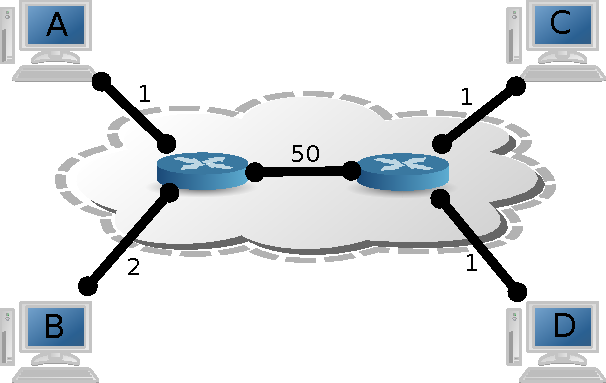
\includegraphics[scale=0.4]{img/algorithms/narada}
%   \label{figure:narada:underlying}
% }\qquad\qquad
% \subfigure[Peer A sends a message to the rest using regular broadcast.] {
%   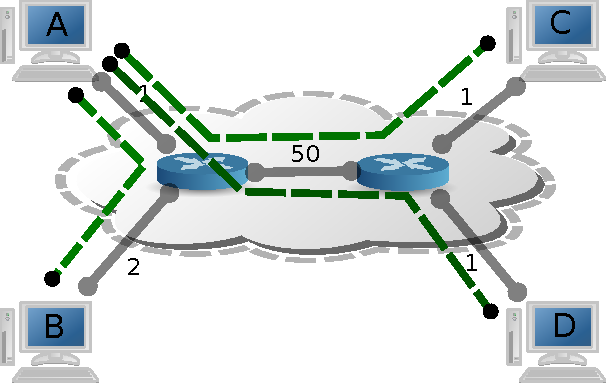
\includegraphics[scale=0.4]{img/algorithms/narada2}
%   \label{figure:narada:regu}
% }\qquad\qquad
% \subfigure[Peer A sends a message to the rest using end system multicast.] {
%   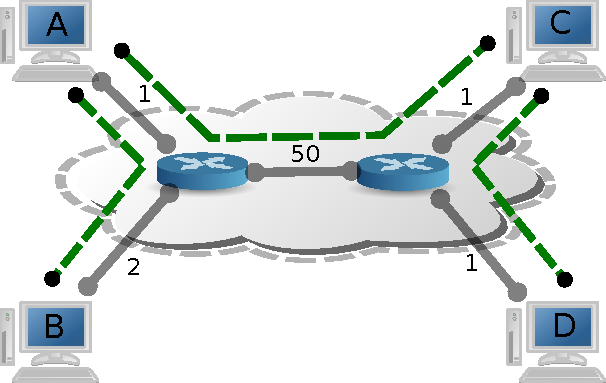
\includegraphics[scale=0.4]{img/algorithms/narada3}
%   \label{figure:narada:multicast}
% }
% \caption{A visualization of the Narada protocol.}
% \label{figure:narada}
% \end{figure}

{\sl Narada}~\cite{CRZ2000,CRSZ2001,CRSZ2002} is a generic
protocol for creating self-adapting overlay networks capable of 
application-layer multicast communications without requiring IP multicast
infrastructure at the network layer.
Although IP--multicast would present a choice in implementing
{\sl Narada}, it is in general considered that it violates the 
stateless design of the current Internet.
Despite the fact the {\sl Narada} was not designed as \p\ system per se,
it was the first to consider the feasibility of overlay-based and application
layer services over the Internet while taking into account 
bandwidth and latency properties of the underlying physical infrastructure.
%%AD you cannot have such a long footnote for God sake!
% \footnote{
  % IP multicast is the term referring to the method of sending IP datagrams to a
  % group of receivers in a single transmission. Even though the method is
  % available some years now, IP multicast has not taken off as anticipated since
  % many believe that it violates the stateless design of the current Internet.
  % For this reason, it is widely deployed in contained environments like
  % enterprises (i.e. IPTV applications - distance learning, video conferencing),
  % commercial stock exchanges, and multimedia content delivery networks.
% }. 
% Although it was not originally designed as a P2P system, Narada is
% a pioneer in that 
% %(and the accompanying \emph{Scattercast} \cite{C2000})
% it was the first to consider the feasibility of overlay-based, application
% layer, services over the Internet that can take into account bandwidth and
% latency properties of the physical underlying infrastructure. 
In the context of this work, the authors came across the 
inefficiency caused by the topology mismatch and attempted to address it 
by building an enhanced connected graph termed \emph{mesh}  %%AD why this graph
							    %% is rich/enhanced???
with each source featuring its own minimum spanning tree.
A gossip-protocol was deployed for the creation of these 
spanning trees~\cite{LYL2008}.
%%
%%AD in general avoid footnotes...  The sentence below does not make sense!
%% "richer" to what???  ENarada is what???
%% 	--- I rephrased as above - not sure correct.. check -----
%% 
% Additionally,
% authors realized the inefficiency caused by the topology mismatch problem and
% tried to address it by building a richer connected graph, called a
% \emph{mesh}, and building per source minimum spanning trees\footnote{
  % ENarada \cite{LYL2008} used Gossip protocol for the
% construction
% }.
%as shown in Figure~\ref{figure:narada}.
Both graph and trees are dynamically updated as nodes keep joining 
or departing the network.
% They also keep the graph and the trees
% dynamically updated while nodes continue to join and leave the network.
The protocol aims to ease the physical link stress, the overall
resource usage as well as the relative delay among end-systems. 
Unfortunately, the main limitation for {\sl Narada} is that 
although it works reasonably well for small groups, 
it does not scale well for larger networks. 
Hence, it is not a suitable choice for potentially large \p\ networks:
%%
\begin{center}
{\footnotesize
\begin{tabular}{ccc}
\emph{Efficiency} & \emph{Overhead} & \emph{Scalability} \\
\hline
%
low &
% The overhead of Narada is proportional to the multicast group size
high &
%
low
\end{tabular}
}
\end{center}

%%%%%%%%%%%%%%%%%%%%%%%%%%%%%%%%%%%%%%%%%%%%%%%%%%%%%%%%%%%%%%%%%%%%%%%%%%%%%%%%
% \subsubsection{Adaptive Overlay Topology Optimization (AOTO)}

Along with {\sl Narada}, the \emph{Adaptive Overlay Topology 
Optimization (AOTO)}~\cite{LZXN2003} is one
of the first attempts to address the topology mismatch problem. 
\emph{AOTO} is a distributed algorithm that seeks to optimize the usage of
the underlying physical resources and operates in $2$ phases:
\emph{Selective Flooding} and \emph{Active Topology}.
In \emph{Selective Flooding}, a minimum
spanning tree is built 
% among  %%AD among???  put "for"...
for each peer and its immediate neighbors so that
queries do not flood the entire network 
% and at the same time 
without simultaneously shrinking their search scope. 
During \emph{Active Topology}, the overlay
links are revised so that they can more closely reflect 
the physical network topology. 
%%
%%AD what is a non-flooding neighbor?
Each peer replaces independently non-flooding neighbors, with closer nodes.
% This is done independently, by each peer by replacing non-flooding
% neighbors, with closer nodes. 
Picking a replacement out of these non-flooding
neighbors follows a random policy called \emph{Randomized AT} algorithm.
To accomplish the above actions, a peer has to keep track of 
its communication costs with all its neighbors (e.g., network delays)
as well as the costs between any pair of neighbors.
%%AD I am not sure what the parenthesis below says.. Rephrased as above
% as well as between any
% pair of neighbors (meaning also that additional, cost probing, message types
% need to be added to the Gnutella protocol). 
The \emph{randomized AT} algorithm is applied by a source peer 
every time its neighbor list is updated or an updated neighbor cost 
table is received.
%%AD do you also obtain neighbor cost tables???
%%
%\paragraph*{Selective Flooding (SF)}
%
% TODO: I DON'T REMEMBER WHY THE FOLLOWING IS MENTIONING LTM WHICH IS ANOTHER
%       ALGORITM. MAYBE THIS CAN BE USED AS A PART OF DISCUSSION AND/OR
%       COMPARISON OF AOTO AND LTM
% TODO: EDIT: LTM SEEMS A MISTAKE HERE BETTER NOT USE IT FOR DISCUSSION (THIS
%             IS AOTO)
%LTM's SF effectiveness has be proven to be detached from the different physical
% or overlay topologies. On the other hand, SF is more effective with large
%number of logical neighbors. It can reach an average optimization rate of 87.4
%percent on a logical topology with an average of 30 logical neighbors.
%
%\paragraph*{Active Topology (AT)}
%
%Different numbers of average logical neighbors has little to do with the
% effectiveness of AT. If the source has $n$ non-flooding peers, there are $n$
%potential neighbor replacements. The overhead to exhaust all $n$ possible
%replacements can be high, so in practice, after each replacement the source
%peer can decide whether it needs to find another candidate peer. This is done
%by computing the cost improvement ratio greater than some predefined
%termination threshold. The larger the threshold, the slower, in the number of
%optimization steps, the reduction of the normalized average distance. As a
%whole the average response time is significantly reduced when more optimization
%steps taken.
%%
\emph{AOTO}'s performance regarding the $3$ criteria is as follows:
%%
\begin{center}
{\footnotesize
\begin{tabular}{ccc}
\emph{Efficiency} & \emph{Overhead} & \emph{Scalability} \\
\hline
%
medium &
% tracking of communication costs to all peer's neighbors as well as between
% any pair of neighbors. Whenever a new neighbor cost table is received or
% there is a change of neighbors, the source peer has to re-calculate the
% multicast tree and apply the randomized AT algorithm.
high &
% needs global knowledge
medium
\end{tabular}
}
\end{center}

%%%%%%%%%%%%%%%%%%%%%%%%%%%%%%%%%%%%%%%%%%%%%%%%%%%%%%%%%%%%%%%%%%%%%%%%%%%%%%%%
% \subsubsection{Adaptive Connection Establishment (ACE)}
The \emph{Adaptive Connection Establishment (ACE)} 
approach~\cite{LZXN2004} uses the network delay as a metric 
to estimate the costs between nodes in a spanning tree.
%%AD when u say spanning tree u mean the ENTIRE network???
Each peer computes the costs to its logical one-hop
neighbors and forms a \emph{neighbor cost table (NCT)} 
using a special routing message type. 
Any pair of neighboring peers exchange their \emph{NCT}s 
and so a minimal overlay topology can be formed.
%%AD the wording of the following is a bit messed up! Simplify! 
%%	reworked as above... check
% Two neighboring peers exchange their \emph{NCT}s in order for
% every peer to obtain the cost between any pair 
% of its local neighbors forming a
% small overlay topology. 
Based on the obtained \emph{NCT}s a minimum spanning tree
for each peer and its one-hop neighbors is created.
%%AD rephrased as above.. This expression "... among each peer" makes 
%%	absolutely NO sense... 
% Moreover, based on obtained NCTs a minimum spanning tree
% among each peer and its one-hop neighbors is built. 
Finally, neighbors located physically far away 
are replaced by physically-closer counterparts. 
In particular, a peer $S$ iteratively probes the distance between 
itself and every of its non-flooding neighbor nodes $G$  as well as 
the distance between $S$ and $G$'s neighbors designated as $H$.
%%AD I do not understand what on earth the following sentence SAYS!!!!
%%	when you say "between" you need to have 2 parties - where is this???
%%	I rephrased as above.. Check correctness...
% Specifically, a peer
% $S$ probes the distance between one of its non-flooding neighbor's neighbors,
% say $G$ and $H$ respectively. 
%%
If the distance between a peer and a neighbor \emph{SG} is measured to 
be larger than that with a neighbor's neighbor \emph{SH}, the link 
between $S$ and $G$ is replaced with a new connection between $S$ and $H$.
%%AD the following is complicated to diff to parse... Tried as above... 
% Assuming that the neighbor's neighbor ($SH$) is
% measured as being ``closer'' than the neighbor ($SG$), the link to the later
% is cut and a new connection is established. 
%%%
%%	%%AD the opposite situation does not appear to be consistent!!!
%	%% with what you say above... 
% In the opposite situation where
% distance $SG$ is closer than $SH$ then if $SH$ is shorter than $GH$, then $H$ is
% preserved as $S$'s new neighbor. 
%%%
%%AD is the distance $GH$ in discussion here as well???  I am confused.
In the case where $SH$ is larger than $SG$ and
$GH$, no connection will be established and $S$ will continue probing another
neighbor's neighbor. 
%%%
The above optimization is conducted within $1$-neighbor
closure using as base a peer and checking all its direct neighbors.
Evidently the scope of such an operation could be extended.
Should  a larger scope be used, a better topology matching can be obtained 
at a greater computational overhead.
%%
%%AD This is NOT English.. No verb??? I am not sure...
% The larger the scope, the better topology matching improvement but
% also the greater the computational overhead.
%
% TODO: SOME DISCUSSION
%
%Simulations in \cite{liu_acesims_2004} show that the average scope of each
% query to cover the same scope of nodes is reduced by about 65 percent without
%losing any autonomy feature, while the average response time can be reduced by
%35 percent. Larger diameter topologies lead to better topology optimization
%rate but also to higher communication and computation overhead. It was also
%found that it is more effective in higher connectivity dense topologies.
%Compared to LTM, it comes short of convergence speed. In
%\cite{ni_mismatch_2004} shows reduction of both total traffic (90 percent) and
%response time (80 percent) to message queries without shrinking the search
%scope.Last but
%not least, it is concluded that work must be done on incorporating a more
%sophisticated selection policy for candidate non-flooding peers.
%

%In \emph{Adaptive Connection Establishment (ACE)} \cite{LZXN2004}, the
%authors extend the idea of AOTO by introducing optimizations based on the
%depths of the minimum spanning trees. But since the network delay is not
%always a reliable estimation method to detect the physical location of peers,
%the algorithm still suffers from the discrepancies caused by mis-located nodes.
%%
%%
\begin{center}
{\footnotesize
\begin{tabular}{ccc}
\emph{Efficiency} & \emph{Overhead} & \emph{Scalability} \\
\hline
% compared to LTM it has slow convergence speed.
medium &
% A little bit better that AOTO since the computation here is done within a
% certain diameter from the source peer
medium &
% Larger diameter topologies lead to better topology optimization
% rate but also to higher communication and computation overhead.
medium
\end{tabular}
}
\end{center}

%%%%%%%%%%%%%%%%%%%%%%%%%%%%%%%%%%%%%%%%%%%%%%%%%%%%%%%%%%%%%%%%%%%%%%%%%%%%%%%%
% \subsubsection{Location-aware Topology Matching (LTM)}


\emph{Location-aware Topology Matching (LTM)}~\cite{LLXNZ2004} 
seeks to optimize an overlay \p\ structure based on the physical topology.
To achieve this, peers issue special messages called
\textit{TTL-detector}s whose \emph{TTL} values are $0$ or $1$;
in this regard, peers 
discover $1$- and $2$-hop neighbor sets ($N$ and $N^2$ respectively) %%AD not 
						%% sure what the N and N2 are..
and proceed to compute communication costs.
% around them and calculating communication costs. 
Time-stamps are used to derive network latency measurements that are then used 
to improve the overlay network without sacrificing the search scope.
% Calculation is achieved through
% timestamp checking, so clocks must be synchronized. 
% The latency information
% gathered is later used to evolve the overlay network into a more efficient one,
% without reducing the search scope. 
Each node compares the latency information
received from its direct neighbors;
peers with longer latencies are placed on a
\emph{will-cut} list where they remain for a certain period of time 
after which they are finally eliminated 
and are placed on the peer's \emph{cut-list}. 
Thus, low-productivity connections are dropped and replaced by 
more efficient ones, reducing the
latency on the overall network. 
Although \emph{LTM} improves the overall efficiency of
the \p\ network, it is unable to offer any warranty for 
effectively addressing the mismatch problem. %%AD shortened and consolidated
%% 
% use real physical topology information,
% just latency metrics, therefore it does not offer a guaranteed safety net for
% the topology mismatch problem.
%
% TODO: SOME DISCUSSION
%
%\paragraph*{Low productive connection cutting}
%There are three cases for any peer $P$ who receives $d(i, S, v)$ multiple
% times:
%\begin{inparaenum}[\itshape i\upshape)]
%  \item $P$ receives both $d(i, S, 1)$ and $d(i, S, 0)$
%  \item $P$ receives multiple $d(i, S, 0)$s from different paths, and P
% randomly chooses to process one
%  \item $P$ receives one $d(i, S, 1)$ and multiple $d(i, S, 0)$s, and $P$
% processes $d(i, S, 1)$ and one randomly selected $d(i, S, 0)$
%\end{inparaenum}
%If the link with the largest cost is found and is a direct neighbor then the
% connection is put in a will-cut list and stays there for a certain period of
%time. If it is not, then it is handled by other peers. After that period,
%connections are cut and recorded to $P$'s cut-list.
%
%\paragraph*{Source probing}
%For a peer $P\in(N^2(S) - N(S))$ who receives only one $d(i, S, 0)$, the cost
% of $PS$ is obtained (with list look-up or probing). Then $P$ compares it with
%the cost from each hop and if $PS$ has the largest cost, $P$ will not keep this
%connection, while otherwise the connection will be created.
%
%\paragraph{}
%Supposing $n$ is the number of peers, $c_n$ is the average number of neighbors
% and $c_e$ is the average cost of logical links, then in the flooding-based
%search the traffic incurred by one query from an arbitrary peer in a
%peer-to-peer network is $O(n)$. As observed in the Gnutella network
%\cite{sripanidkulchai_gnutella_2001}, each peer issues $0.3$ queries per minute
%in average, thus the per minute traffic incurred by the network with $n$ peers
%is $O(n^2)$. Because each $d(i, S, v)$ has a TTL of $2$ in each source peer,
%the traffic for one time LTM optimization in all peers is at most $2nc_n^2c_e$.
%If each peer uses LTM $k$ times per minute, the total traffic incurred is
%$2knc_n^2c_e$. Simulation shows the best value for $k$ is $2$ or $3$. So, the
%traffic overhead caused by LTM to the network is $O(n)$.
%
%TTLj-detectors, with $j > 2$, would detect and break cycles with more than 4
% links. LTM though, does not use such detectors because detector-flood traffic
%would increase significantly, and cut links between two end-peers, could cause
%queries initiated by them to traverse a path much more expensive than the cost
%on the the cut link.
%
%\paragraph{}
%LTM disadvantages are
%\begin{inparaenum}[\itshape i\upshape)]
%  \item disagreement of measured delay due to unsynchronized clocks causes
% problems when deciding the cut positions, which can influence the network
%connectivity, and
%  \item the network delay metric mainly focuses on disabling the connections
% between peers physically far away without considering the shortcuts created by
%powerful peers.
%\end{inparaenum}
%
\emph{LTM} fares as follows regarding our $3$  criteria:
\begin{center}
{\footnotesize
\begin{tabular}{ccc}
\emph{Efficiency} & \emph{Overhead} & \emph{Scalability} \\
\hline
% Authors claim 75% reduction on traffic cost and about 65% reduction on query
% response time.
medium &
%
medium &
%
medium
\end{tabular}
}
\end{center}

%%%%%%%%%%%%%%%%%%%%%%%%%%%%%%%%%%%%%%%%%%%%%%%%%%%%%%%%%%%%%%%%%%%%%%%%%%%%%%%%
% \subsubsection{Scalable Bipartite Overlay (SBO)}

The \emph{Scalable Bipartite Overlay (SBO)}~\cite{LXN2004,LXN2007} 
reduces the overhead of creating
and maintaining a minimum spanning tree 
by randomly dividing the nodes into
two groups --\emph{red}s and \emph{white}s-- 
and assigning different tasks to the two groups.
When a peer joins the network, it is randomly assigned with an initial
color (red or white).
%  (separating all peers into two groups). 
Then the network bootstrap host node furnishes the joining peer with a list
of active peers along with their color information. 
%%AD how many nodes are provided here??? 
The joining peer uses this list to 
establish connections to differently colored peers. 
In this regard, all peers form a a bipartite overlay. 
Using the network delay as a metric, white-peers 
peers measure distances from red counterparts
and report the encountered red neighbors.
Having information on all their $2$-hop neighbors 
($N^2$) %%AD I am not sure what this N^2 means here!
red-peers create minimum spanning trees for the neighbors in question and
% assigns %%AD this should be plural
assign efficient forwarding paths. 
Having a minimal $2$-hop spanning tree, 
a red-peer dispatches its queries only within this range. 
Some white-peers, though, may have become non-forwarding neighbors. 
%%AD I am not sure how you reach the above sentence... 
%%
%%AD The following sentence is very convoluted. I cannot parse it!
In this phase, such a (white) neighbor will try to find another 
red peer being two hops away from its
current red neighbor to replace the later as its new neighbor. 
%%%%
The white-peers can further optimize their positions within 
the overlay if this is required. 
%%AD What are the implication of the above statement?? 
%%   What is the end result of the approach in terms of the mismatch problem??? 
%%   Something is missing... 
%
% TODO: SOME DISCUSSION
%
%In a static environment LTM may reduce traffic cost by around 80 to 85 percent
% while SBO reduces traffic cost between 85 and 90 percent. However, LTM  is
%proved to converge in around 2-3 steps while SBO needs 4-5 steps. Moreover LTM
%reduces response time by more than 60 percent in 3 steps while SBO needs 8. In
%a dynamic environment (10 minute average peer lifetime, 0.3 queries/sec by each
%peer) SBO and LTM reduce the average traffic cost per query (including the
%overhead due to the optimization steps) by 85 and 80 percent, respectively.
%Moreover LTM reduces the response time per query to 30 percent while SBO to 35
%percent.
%
%\cite{ni_mismatch_2004} shows SBO, achieves approximately 85 percent reduction
% on traffic cost and about 60 percent reduction on query response time.
In regards to the $3$ stated criteria, \emph{SBO} behaves as follows:
\begin{center}
{\footnotesize
\begin{tabular}{ccc}
\emph{Efficiency} & \emph{Overhead} & \emph{Scalability} \\
\hline
% SBO reduces traffic cost between 85 and 90 percent
high &
% compared to LTM it has slower convergence speed thus incurs more, total,
% overhead.
medium &
%
medium
\end{tabular}
}
\end{center}

%%%%%%%%%%%%%%%%%%%%%%%%%%%%%%%%%%%%%%%%%%%%%%%%%%%%%%%%%%%%%%%%%%%%%%%%%%%%%%%%
% \subsubsection{Two-Hop-Away Neighbor Comparison and Selection (THANCS)}

The distributed heuristic termed 
\emph{Two-Hop-Away Neighbor Comparison and Selection (THANCS)}~\cite{LNXE2005,L2008} attempts to minimize overlay hop costs.
\emph{THANCS} is essentially a \emph{local search method} as it aims 
to find a locally optimum solution by exploiting knowledge within 
a $2$-hop radius. 
The algorithm consists
of two main components: \emph{piggybacking neighbor distance on queries} and
\emph{neighbor comparison and selection}.

The \emph{piggybacking component} requires peers 
to probe immediate neighbors using delay distance measurements 
and store information locally. 
This is done by introducing a special query message type, the
\emph{Piggy Message (PM)} which includes information about 
the neighbor identification and measured distance. 
A peer $p$ constructs a \emph{PM} for its
neighbor $n$, which contains $n$'s IP address and the distance between them.
%%
If $p$ receives a query from $n$, the respective \emph{PM}-message will 
be piggybacked to the query and $p$ will forward this enlarged message to
of its neighbors.
% When $p$ receives a query from $n$, this PM will be piggybacked to the query
% message that will be then forwarded to all other neighbors of peer $p$. 
In turn, each neighbor $q$ will detach the \emph{PM}-information,
% (it will not be further forwarded) 
record the distance $pq$ and further process the query. %%AD added "further" - correct??
%%%
%%AD rephrased as above... When you use "this" "that" etc BE careful...
% Each neighbor will detach the PM information 
% (it will not be further forwarded),
% record the $pq$ distance and process the query 
% as always after receiving a query message.  %% THIS "as... " threw me off!!!!
%%%%%%%%%%%%%%%%%%%%
Selection of which incoming queries should piggyback a \emph{PM} is proposed
by either \emph{pure probability-based (PPB)} or \emph{new neighbor triggered
(NNT)} policies. 

The \emph{neighbor comparison and selection} component
helps peer $p$ probe all his neighbors placed upto 
$2$-hops away ($ N^2(p)$) %%AD what is this?? complexity???
not probed so far.
The distance of $pn$ is known to $p$. %%AD I am not sure what you say!
Upon receiving a \emph{PM} from node $n$ with the distance of $nq$, 
where $q$ is a direct
neighbor of $n$, $p$ chooses one of the following two paths. 
\begin{itemize} %%AD put the two directives here...
\item[--]
	if $q$ is a $1$-hope neighbor of $p$, then 
	$p$ 
\item[--]
\end{itemize}
%%AD I cannot follow what on earth it is said here... this needs 
%%	rewriting and better structuring..  Use the above list for 
%%	the expected operation...
First, if $q$ is a
direct neighbor of $p$, then the latter will check the cost of the involved
links. If the most cost-intensive link is one of $pq$ or $pn$, then it is put
into a \emph{will-cut} list. If it is $nq$ then nothing is done (since either
$n$ or $q$ will have the chance to handle it themselves).  
%%AD this is what I think should go into the second clause above... 
On the other hand, if
$q$ is within two-hop radius from $p$, the later probes the former (if it hasn't
got the distance information yet) and again compares distances $pq$, $pn$, and
$nq$. If $pq$ is the most cost-intensive, $p$ will not establish the connection.
If it is $pn$, $p$ will establish connection $pq$ and put $pn$ in the will-cut
list. 
If it is $nq$, $p$ will stay connected with both $n$ and $q$,
such that eventually in later stages either $n$ or $q$ will disconnect link $nq$.  
%%AD The above paragraphs need clearing up.. The text cannot be read.. 
%%
%%AD Also, make the connection with the mismatch problem... and justify 
%%	somewhat convincingly why the rating below comes true...
%
% TODO: SOME DISCUSSION
%
% \begin{inparaenum}[\itshape i\upshape)]
%   \item is completely distributed and needs no global knowledge,
%   \item presents trivial overhead compared to the query cost savings
%   \item its convergent speed of the algorithm is fast enough (faster than
% minimum spanning tree approaches) so that is effective to dynamic
% environments, and
%   \item does not shrink the search scope.
% \end{inparaenum}
%
%In a static environment THANCS has been proven to be effective; optimizing 45
% percent out of the 60 percent of mismatched paths, constructing a nearly
%optimal overlay. This leads to a 60 percent reduction in traffic cost as well
%as a 40 percent decrease in query response time. In dynamic environments
%(Gnutella 0.6/Limewire super-peer-like and Ion flat-like), THANCS saves up to
%70 percent of the traffic cost in the super-peer topology and 55 percent for
%the flat one. Average response time is also decreased by 60 and 45 percent,
%respectively. Generally, THANCS has similar performance to LTM, without needing
%synchronization. SBO, incurring half the  overhead of AOTO, reduces the traffic
%cost the most, while THANCS has lower response time and converges faster than
%SBO. THANCS is, thus, more suitable for a more dynamic environment. In
%addition, THANCS is easy to implement and its operation overhead is trivial,
%compared with the other three approaches. This design, however, has the
%limitation of not being easily extend to also support non-flooding-based
%systems.
\begin{center}
{\footnotesize
\begin{tabular}{ccc}
\emph{Efficiency} & \emph{Overhead} & \emph{Scalability} \\
\hline
% 
medium &
% trivial overhead compared to the query cost savings and its convergent speed
% is faster than minimum spanning tree approaches so less overall overhead cost.
low &
% completely distributed and needs no global knowledge,
high
\end{tabular}
}
\end{center}

%%%%%%%%%%%%%%%%%%%%%%%%%%%%%%%%%%%%%%%%%%%%%%%%%%%%%%%%%%%%%%%%%%%%%%%%%%%%%%%%
The \emph{Hops Adaptive Neighbor Discovery (HAND)} algorithm~\cite{CLZHC2006}
uses a fully-distributed triple--hop adjustment strategy
to address the topology mismatch problem.
\emph{HAND}'s goal is to shape the current overlay
graph $G$ into an optimal \emph{Logical Communication Network} 
%(LCN)} %%AD why u need this acronym? u never use it!
$G^{*}$.
% \subsubsection{Hops Adaptive Neighbor Discovery (HAND)}
% \cite{CLZHC2006} proposes the \emph{HAND} algorithm which uses a
% fully distributed triple hop adjustment strategy to address the topology
% mismatch problem. The approach's ultimate goal is to shape the current overlay
% graph $G$ into the \emph{Logical Communication Network (LCN)} $G^{*}$ which is
% how the optimal overlay is referred in the paper's context. 
This optimality is attained if all peer hop 
sequences $(v_1, v_2, \ldots, v_k)$ of $G$ exist in $G^{*}$ 
and are in the same order.
The latter indicates that in 
practice triple sequences $(v_1, v_2, v_3)$ are used.
%%AD this used to be a footnote - avoid footnotes in general!
%%
A mismatch is detected as follows:
suppose we want to verify peer a
sequence, say $v_2-v_1-v_3$. 
Two probing messages are dispatched from $v_1$ to
$v_2$ and $v_3$ and yield delays of $x$ and $z$ respectively.
%
When the probing message arrives at $v_2$, it gets forwarded
directly to $v_3$. 
Similarly, the message reaching $v_3$, it is directly forwarded to $v_2$.
The above two forwarding actions seek to quantify 
the corresponding delays of $(v_2,v_3)$ and $(v_3,v_2)$ physical paths
denoted by $y$. 
%%
If $y=z-x\pm\varepsilon$, the sequence $v_2-v_1-v_3$ is mismatched and should
be adjusted to $v_1-v_2-v_3$ by deleting edge $(v_1,v_3)$ and 
then adding a new $(v_2,v_3)$. 
If $y=x-z\pm\varepsilon$, sequence $v_2-v_1-v_3$ is mismatched and
should be adjusted to $v_1-v_3-v_2$ by deleting edge $(v_1,v_2)$ and adding a
new $(v_3,v_2)$. 
The  $\varepsilon$ is a small positive real number denoting
additional delays caused by possible forwarding and jitter delays. 
%%
The advantages of \emph{HAND} are that it
\begin{inparaenum}[\itshape i\upshape)]
  \item does not need any clock synchronization,
  \item is a fully distributed algorithm.
  \item involves low traffic overhead,
  \item can be used in dynamic \p\ environments, and 
  \item furnishes low query response times.
\end{inparaenum}
%
% TODO: SOME DISCUSSION
%
%Measurements conducted for evaluation purposes showed that in a static
% environment the algorithm can effectively decrease traffic cost by about 77
%percent and shorten the query response time by about 49 percent in less than
%two minutes. In a dynamic environment it shows similar behavior and with the
%size of the overlay network having little impact on the effectiveness of the
%algorithm. Compared to LTM both algorithms have almost the same traffic
%reduction rate, however on the response time reduction rate HAND has a higher
%one by about 4 percent. The traffic overhead of HAND is much less than that of
%LTM by an average of 55 percent.
In terms of the $3$ stated criteria, \emph{HAND} fares as follows:
\begin{center}
{\footnotesize
\begin{tabular}{ccc}
\emph{Efficiency} & \emph{Overhead} & \emph{Scalability} \\
\hline
% similar traffic reduction rate savings to LTM
medium &
% The traffic overhead of HAND is much less than that of LTM by an average of
% 55 percent.
low &
% no clock syncing needed, fully distributed and with low control overhead the
% algorithm can be considered scalable.
high
\end{tabular}
}
\end{center}

%%%%%%%%%%%%%%%%%%%%%%%%%%%%%%%%%%%%%%%%%%%%%%%%%%%%%%%%%%%%%%%%%%%%%%%%%%%%%%%%
% TODO: DOUBLE CHECK IF THIS ALGORITHM GOES IN THIS SECTION/SUBSECTION
% \subsubsection{Adaptive Peer Selection (APS)}
The \emph{Adaptive Peer Selection (APS)} approach uses 
machine learning techniques to form peer
selection strategies based on past experience~\cite{BFLZ2003}. 
A decision tree is used to rate peers based on information 
collected for the characteristics of established connections.
Such features include load, bandwidth, and past uploading experience. 
%%AD load on what?? The dispatching end? the receiving end??
Subsequently, a Markov decision process is introduced 
as a mechanism to shape the policy
for switching among the peers. 
The success of approach depends on how fast the introduced 
peer selection functions. Admittedly, \emph{APS} is slow 
due to the learning process and its inherent complexity.
As far as the $3$ criteria is concerned, \emph{APS} has as follows:
\begin{center}
{\footnotesize
\begin{tabular}{ccc}
\emph{Efficiency} & \emph{Overhead} & \emph{Scalability} \\
\hline
% machine learning the best way to adapt the overlay 
high &
% high computation overhead for learning and very slow convergence speed for
% the learning process.
high &
%
low
\end{tabular}
}
\end{center}

%%%%%%%%%%%%%%%%%%%%%%%%%%%%%%%%%%%%%%%%%%%%%%%%%%%%%%%%%%%%%%%%%%%%%%%%%%%%%%%%
The \emph{Innocuous Topology Aware Overlay Construction (ITA)} approach~\cite{PRFM2009} seeks to offer both an overlay formation approach and furnish 
an effective way to carry out searching.
% \subsubsection{Innocuous Topology Aware (ITA) Overlay Construction}
% \cite{PRFM2009} introduces an algorithm for Innocuous Topology Aware
% construction of unstructured P2P networks. The paper's proposition is twofold.
% Overlay construction and search method. 
When constructing the overlay, \emph{ITA} exploits the notion of 
of \emph{short} and \emph{long} connections.
% For the overlay construction, it employs
% the notion of \emph{short} and \emph{long} connections. 
Should $N$ be the number of network peers, 
$\alpha \leq 1 $ a system-wide magic number
and $x$ an $\alpha$-related latency threshold,
the bootstrapping peer randomly selects $\alpha \ast N$ 
``close'' (latency below $x$) and 
$\left( 1 - \alpha \right) \ast N$ distant (latency above $x$) nodes
as its neighbors. 
%%AD how do they select all these magic constants???
%%
Searching occurs in two phases: in the initial phase, the querying node
floods its distant neighborhood  with $TTL = 1$.
Subsequently, peers receiving a query over a ``long link'' commence a 
local flood with $TTL\;=\;ttl$ where \emph{ttl} is system-defined.
%%AD how are you supposed to define these params?? in a fixed manner?? 

The main objective of the overlay construction phase
is to yield a network that exhibits low clustering. 
In turn, this is 
a beneficial characteristic for random graphs as it can lead to a
larger coverage of peers with the same number of messages and 
at the same time helps reduce duplication. 
%%AD same number of messages in comparison to what?? 
%%	same: duplication of what?? messages right???
This combination offers efficient lookups that pose minimal 
or no negative impact to other mechanisms possibly employed by 
the \p\ systems.
% This means more efficient information lookup that has minimal or no
% negative impact whatsoever to the rest of the mechanisms employed in
% unstructured P2P systems\footnote{For example the 1-hop replication and the
% dynamic querying mechanisms of later versions of Gnutella.}. 
A 50\% reduction in communication latency among peers by cutting off 
some 20\% of the \emph{IP}-level traffic generated 
in reported in~\cite{PRFM2009}.
%%
\emph{ITA} places as follows in the context of the $3$ criteria:
%
\begin{center}
{\footnotesize
\begin{tabular}{ccc}
\emph{Efficiency} & \emph{Overhead} & \emph{Scalability} \\
\hline
% low clustering with larger coverage of peers with the same number of messages
% and reduced duplication.
medium &
% construction at peer join, while searching using local ``floods''
low &
% the selection of neighbors is done at join time. No overlay adaptation means
% low scalability in dynamic environments.
medium
\end{tabular}
}
\end{center}

%%%%%%%%%%%%%%%%%%%%%%%%%%%%%%%%%%%%%%%%%%%%%%%%%%%%%%%%%%%%%%%%%%%%%%%%%%%%%%%%
% \subsubsection{EGOIST}
\emph{EGOIST}~\cite{SLLBBR2008} is a set of algorithms 
to construct and manage overlay networks. 
\emph{EGOIST} utilizes a selfish approach in the sense that every participating
peer continuously updates its neighbors so as to minimize the sum of distances
to all destinations under shortest-path routing. 
A newly arriving peer, randomly connects to an already participating 
node through a bootstrap server. 
Once connected, the peer starts receiving information throughout the
link-state mechanism and thus, after some time, 
it has a complete picture of the overlay graph. 
Then the peer estimates the delay to all other nodes to
determine its potential neighbors and ultimately connects 
to the overlay using some policy; such a policy might be 
for example the minimization of the average delay to all its
neighbors. 
\emph{EGOIST} requires extensive resource usage to continuously update the
wiring of all the nodes in the system. 
%%AD I am not sure I get the "wiring of all"??? clarify.. 
The approach can reduce the load imposed by the monitoring 
and announcing process from $O(n^2)$ to only $O(kn)$, 
where $n$ is the number of all network nodes 
and $k$ is the number of links a node chooses to establish.
%%AD is this an average number?? What kind of number???
Regarding the $3$ criteria, \emph{EGOIST}'s behavior is as follows:
\begin{center}
{\footnotesize
\begin{tabular}{ccc}
\emph{Efficiency} & \emph{Overhead} & \emph{Scalability} \\
\hline
% peer neighborhood selected to minimize, for example, average delay
high &
% link state info (heartbeat) and delay estimation to all other nodes
% resulting to a complete picture of the overlay graph.
high &
% need global knowledge
low
\end{tabular}
}
\end{center}

% TODO: CHECK IF THE FOLLOWING BITTORRENT ALGORITMS BELONG IN THIS SUBSECTION
%%%%%%%%%%%%%%%%%%%%%%%%%%%%%%%%%%%%%%%%%%%%%%%%%%%%%%%%%%%%%%%%%%%%%%%%%%%%%%%%

The main objective of the \emph{Biased Neighbor Selection (BNS)} 
approach~\cite{BCCMSBZ2006} is to 
strengthen {\sl BitTorrent}'s~\cite{c_bittorrent_2003} locality 
by carefully choosing most of the neighbors of a peer to come from 
the same \emph{ISP} while at the same time adhering to the near-optimal
download performance of the protocol.
%%
By and large, {\sl BitTorrent}s deploy mechanisms that have proved 
aggressive for \emph{ISP}s' networking and accounting as they function 
in a ``without-borders'' approach.
% BitTorrent systems employ most of the time
% mechanisms that can be proven very aggressive to an ISP's networking and
% accounting, basically, due to their lack of knowledge of Autonomous System
% boarder limits. 
The default {\sl BitTorrent} specification designates $35$ connections 
for each peer regardless if such connections are placed within or outside 
the borders of the \emph{ISP} that hosts the node.
%%
\emph{BNS} proposes that only $k$ out of these $35$ connections are 
established with nodes beyond the {\it ISP}-borders;
the $k$ connections offer an extended and ``global'' view of 
the network at large and seek to strike a balance between 
the load imposed inside and outside the \emph{ISP}.
The latter refrains peers from exchanging traffic through
expensive network links should there exist alternative local connections
offering the sought services.
%%AD rewrote as above...
% Biased neighbor selection experiments on some number $k$ which
% denotes a number of neighboring peers which are not on the same ISP than the
% peer at hand. 
% Consequently, the remaining $35 - k$ peers are from the same ISP.
% These $k$ nodes are used to provide a more extended, global view of a
% network, but balance the load within the limits of a single ISP.
% This prevents clients from exchanging traffic through an expensive transit link,
% if there are alternative local connections that could offer the same service faster and
% at no additional cost for the ISP. 
\emph{BNS} is realized either through 
the modification on the tracker so that \emph{ISP}-local resources are rapidly 
identified,
or through \p\ traffic shaping devices installed on \emph{ISP} edge routers. 
%%
In~\cite{BCCMSBZ2006}, a combination of 
biased neighbor selection along with bandwidth throttling
and caching techniques for near-optimal lookup results is proposed.
% The paper also proposes
% a combination of biased neighbor selection along with bandwidth throttling and
% some caching techniques for near optimal results. 
%%%%%%%%%%%%%%%%%%%%%
% Unfortunately, implementation
% and deployment
% need knowledge of ISP Autonomous System mappings %%AD What are these Aut. Sys?
% or infrastructure changes (installation of P2P traffic shaping devices) on the
% ISP, making widespread adoption.
%%AD I am not sure what the above sentence says! I rephrased as follows:
Unfortunately, \emph{BNS} deployment requires knowledge of 
\emph{ISP} network mappings and awareness of possible changes 
that occur in the infrastructure limiting its widespread adoption;
the following table qualitatively depicts the expected behavior of \emph{BNS}:
%%
\begin{center}
{\footnotesize
\begin{tabular}{ccc}
\emph{Efficiency} & \emph{Overhead} & \emph{Scalability} \\
\hline
% inter-ISP cost minimized while retaining the near optimal performance of
% BitTorrent download.
high &
% this info is taken at swarm join
low &
% trackers should maintain and update proximity info/proximity info is
% retrieved from special hardware.
medium
\end{tabular}
}
\end{center}

%%%%%%%%%%%%%%%%%%%%%%%%%%%%%%%%%%%%%%%%%%%%%%%%%%%%%%%%%%%%%%%%%%%%%%%%%%%%%%%%
\emph{Ono}~\cite{CB2008} is a protocol that helps contain
{\sl BitTorrent} traffic within individual \emph{ISP}s
and enhances the downloading rates by favoring connections
within the borders of a single autonomous system.
% \subsubsection{Ono}
% Choffnes and Bustamante propose Ono \cite{CB2008}, a protocol for managing
% BitTorrent traffic so that it significantly reduces cross-ISP traffic and at the
% same time enhances downloading rates by favoring connections within the borders
% of a single autonomous system. 
Contrary to \emph{BSN}~\cite{BCCMSBZ2006},
\emph{Oro} leads to improved performance 
without requiring any explicit cooperation between 
\emph{ISP} subscribers or any additional
infrastructure and network topology information.
% Contrary to biased peer selection proposed in
% \cite{BCCMSBZ2006}, this work can lead to 
% improved performance without requiring
% any cooperation between ISP subscribers, or requiring any additional
% infrastructure and network topology information. 
\emph{Oro}'s selection approach is 
landmark-based and leverages existing {\sl CDN}-infrastructure 
for peer distance estimation. 
%%AD I do not understand the following sentence... I am not even sure what 
%%   who is close to each other??? Confusing sentence. Rephrase...
{\sl CDN}s already use both static (i.e., geographical) and dynamic
(network measurement systems) information for their replica selection, so the
authors claim that peers which exhibit similar redirection behavior, are 
likely close to the replica servers and as a consequence close to each other.
%%
The redirection behavior is modeled in terms of \emph{ratio map}, 
a vector of \emph{$<$replica-server,ratio$>$} tuples, where \emph{ratio} is
the percentage of times the {\sl CDN} redirects the peer 
to the specific \emph{replica-server}.
%%
The bootstrapping phase %%AD of what?? the protocol's bootstrapping???
consists of the peer performing {\sl DNS} lookup to {\sl CDN}-names
%%AD when you say "CDN names" - what are they????
to build its redirection information.
%%
Initially, the {\sl DNS} polling interval is set to $30$ seconds 
and increases by $1$ minute every time redirection information 
to the {\sl CDN} remains unchanged after the lookup.
The {\sl DNS} polling interval is halved if pertinent 
redirection information has changed.
To avoid the bootstrapping phase when the \emph{ratio map} 
is sufficiently fresh, 
\emph{Oro} persists the information 
after the end of a BitTorrent session.
%%AD what information is this?? DNS look ups?? 
%%
\begin{center}
{\footnotesize
\begin{tabular}{ccc}
\emph{Efficiency} & \emph{Overhead} & \emph{Scalability} \\
\hline
% Authors claim minimization of inter-ISP traffic cost while enhancing the,
% already, near optimal performance of BitTorrent download.
high &
% periodic DNS lookups and CDN redirection imposes medium control overhead to
% the method.
medium &
% the use of CDNs make the approach not fully distributed thus less scalable
low
\end{tabular}
}
\end{center}

%%%%%%%%%%%%%%%%%%%%%%%%%%%%%%%%%%%%%%%%%%%%%%%%%%%%%%%%%%%%%%%%%%%%%%%%%%%%%%%%
Three approaches that ``inject'' locality awareness 
in {\sl BitTorrent}-like applications are discussed in~\cite{LCLX2009}.
% \subsubsection{Locality-Awareness in BitTorrent-like P2P Applications}
% In \cite{LCLX2009} the authors study and compare three different
% approaches in injecting locality awareness in BitTorrent-like applications. 
The first \emph{macroscopic-level} approach 
focuses on improving the neighbor selection process. 
When a peer asks a tracker to join, 
the later sorts its swarm peers according to
their hop-count distance from the requesting peer 
send out the top-$k$ list of nodes (e.g., $k$=$50$).
%% Autonomous System  hope distance... 
%%AD Got this out - do u need it?? What does it mean "Autonomic System Hop Dist"???
%%
The second approach manipulates the {\sl BitTorrent} chocking/unchocking.
% at an \emph{intermediate-level}. 
A peer unchockes its $4$ closest in terms of 
% Autonomous System 
hop-count interested neighbors. 
The same applies also when the peer turns to 
the seeding state;  this  \emph{intermediate-level} approach favors
least distance and is in contrast to the original {\sl BitTorrent} 
implementation which favors uploading speed.
%%
Finally, the third approach that operates at 
a \emph{microscopic-level}, substitutes the rare-first chunk picking
policy by a locality-first policy. 
%%AD is it "rarest"?? What does it mean "locality-first"???
The distance value of a piece is computed as the mean value 
of the distances of the peers that posses it. 
%%AD What is this "piece"??? I am not sure how the average gets computed? 
%%   It is very cryptic description...
Through experimentation, %%AD simulation? real?
the locality-based approach achieves traffic optimization.
Nevertheless, it does not do that well when compared with the 
random approach of the standard {\sl BitTorrent} protocol.
%%AD rephrased and shortened the following as above...
% The paper conducts several measurements on the efficiency of this scheme 
% and reaches 
% the conclusion that the major design decision for all locality
% aware P2P systems is the trade-off of optimizing inter- Autonomous System
% traffic versus achieving fairness amongst peers.  While their
% locality-based approach achieves traffic optimization, it does not do well
% when compared with the 
% random approach of the standard BitTorrent protocol.
%%%%%%
%%AD so in general how does this approach help the mismatch problem?? 
%%	need a statement here (1-2 sentences explaining this).
\begin{center}
{\footnotesize
\begin{tabular}{ccc}
\emph{Efficiency} & \emph{Overhead} & \emph{Scalability} \\
\hline
% minimization of inter-AS traffic but unfair among peers.
medium &
% info (AS hop distances) acquired at swarm join
low &
%
high
\end{tabular}
}
\end{center}

%%%%%%%%%%%%%%%%%%%%%%%%%%%%%%%%%%%%%%%%%%%%%%%%%%%%%%%%%%%%%%%%%%%%%%%%%%%%%%%%
\emph{TopBT}~\cite{RTLCGZ2010} seeks to enhance 
proximity awareness in the {\sl BitTorrent}
without the need of any additional infrastructure.
% \subsubsection{TopBT}
% \cite{RTLCGZ2010} proposed an approach for enhancing proximity awareness
% in the BitTorrent protocol without any need of any infrastructure installed. 
The key conjecture upon which \emph{TopBT} is built is that 
a good peer selection metric should take into account both the
downloading speed and the network topology. 
In this context, the approach suggests a metric that designates
peers demonstrating high download rate, low reciprocal upload demand 
and low routing hops.
The metric is defined as the ratio of download to upload rate ${d}/{u}$
divided by the either the link-level $l$ or the number of routing hops required $a$.
%%AD The following is not a readable sentence... rephrase as above...
% Thus, it proposes the use of the
% ratio of download rate to upload rate, $\frac{d}{u}$, divided by link-level or
% Autonomous System -level routing hops, $l$ or $a$ respectively, in an attempt to
% form a comprehensive metric to select peers with high download rate, low
% reciprocal upload demand and low routing hops.  %%AD What is "Autonomous System -level routing hops?????"
%%%%%%%%%%%%%%%%%%%%%%%%
The above \emph{TopBT}-metric is applied in various
aspects of the original {\sl BitTorrent} protocol to ``inject'' topology
awareness for improved peer selection. 
%%
In a effort to essentially improve on the inherent topology mismatch problem,
\emph{TopBT} modifies the peer list the
tracker returns when someone first tries to connect to the swarm,
the initial connection establishment, and the
unchoking mechanism in the {\sl BitTorrent}.
%%AD how do they specifically are modified??? What is the difference 
%%	with the previous paper?
%%
%
%
%A peer that runs the TopBT protocol evaluates its neighbors by periodically
%emitting pings or trace-routes in order to unchock those peer that exhibit less
%hops to reach and higher download rates. \emph{Link-hops} are measured by using
%the TTL value that the originator receives as a response from the remote
%peer\footnote{Initial TTL values are known for the different operating systems
%(e.g. 64 for Linux or 128 for Windows NT/2000/XP) so the originator can
%calculate the hops using the value of the TTL on the response message it
%receives.}. Also the peer, when off-line, builds a table that maps IPs to
%\emph{AS-hops}, using BGP dumps.
%%
Through experimentation on hundreds of {\it PlanetLab} and residential hosts,
\emph{TopBT} offers more than 25\% traffic reduction and 15\% faster downloads
if compared with popular {\sl BitTorrent} implementations.
%%AD rephrased what is below as above ...
% the authors claim more than 25\% traffic reduction and 15\% faster downloads,
% both with a lightweight cost when compared to popular BitTorrent
% implementations.
%
In reference to the stated $3$ criteria, \emph{TopBT} fares as follows:
\begin{center}
{\footnotesize
\begin{tabular}{ccc}
\emph{Efficiency} & \emph{Overhead} & \emph{Scalability} \\
\hline
% it takes into account both dl speed and network topology. The later though is
% rather coarse grained since it is taken into account on the AS level.
medium &
% the algorithm does not involve extensive calculations.
low &
% Does not need infrastructure and the calculations are distributed so it can
% scale
high
\end{tabular}
}
\end{center}

%%%%%%%%%%%%%%%%%%%%%%%%%%%%%%%%%%%%%%%%%%%%%%%%%%%%%%%%%%%%%%%%%%%%%%%%%%%%%%%%
The \emph{Underlying Topology-Aware Peer Selection (UTAPS)}~\cite{LCY2008}
is an effort to furnish an enhanced peer selection strategy.
% \subsubsection{Underlying Topology-Aware Peer Selection (UTAPS)}
% UTAPS \cite{LCY2008} is another peer selection strategy for the BitTorrent
% protocol. 
\emph{UTAPS} essentially works in two stages: in the first,
it collects information to develop a picture of the underlying topology 
and in the second, it proceeds to make the peer selection based on 
this knowledge.
In the first stage, \emph{UTAPS} employs
network tomography, a technique that probes from a large network's 
endpoints to infer its internal characteristics~\cite{chny_tomography_2002}. 
%%
Upon arrival of a new peer, the tracker trace-routes 
it to obtain some basic knowledge 
including IP address, routers involved, \emph{RTT} and number of 
hops traversed.
The more the peers in the swarm the better 
picture a tracker has for the underlying infrastructure.  
The tracker provides this information to the newcomer in the form
of the bootstrapping peer list. 
%%
%%AD I am lost among the peers in the following sentence... Who traces whom???
The peers further enhance this picture by
trace-routing the returned peers themselves and reporting back to the tracker.
%%
In the second stage,  \emph{UTAPS} employs a set of heuristics
which target those peers that expose low \emph{RTT}
and are found within certain hop-counts away from 
observed routers. %%AD u had "measured routers" - how do you select these routers?
% For the selection part, a family of heuristics are proposed, which in general
% target those peers that expose low RTT and are within certain hop-count away of
% measured routers. 
%%
%%AD if you leave this "the authors claim..." and an such an author gets 
%%	to spend 30 secs with the paper, you are dead! dead dead!!! 
%%
% The author's claim that peers running UTAPS instead of random
% peer selection can achieve better downloading rates with reduced burden on the
% underlying ISP infrastructure though their technique is coarse-grained and their
% evaluation configuration was far too small for extracting further safe
% conclusions.
It is reported in~\cite{LCY2008} that peers running \emph{UTAPS}
instead of the random peer selection, achieve better downloading rates
and at the same time offer reduced burden on the underlying \emph{ISP}s. 
\emph{UTAPS} stands as follows in regard to the $3$ criteria:
%%
\begin{center}
{\footnotesize
\begin{tabular}{ccc}
\emph{Efficiency} & \emph{Overhead} & \emph{Scalability} \\
\hline
% coarse grained approach of the network tomography doesn't provide a detailed
% picture of the underlying network that the peers can then exploit
medium &
% trace-route and hop counts and calculation from both the tracker and the peers
% (the later for all peers in the bootstrapping list) increases the control
% overhead of the approach.
medium &
%
medium
\end{tabular}
}
\end{center}

%%%%%%%%%%%%%%%%%%%%%%%%%%%%%%%%%%%%%%%%%%%%%%%%%%%%%%%%%%%%%%%%%%%%%%%%%%%%%%%%
A clustering approach that differentiates peers encountered in a swarm
in those that are local, intra-\emph{ISP} and inter-\emph{ISP} is 
presented in~\cite{QLZG2009}.
The classification is carried with the help of the routers used 
while peers communicate with the tracker.
% \subsubsection{An Effective Network-Aware Peer Selection Algorithm in
% BitTorrent}
% Qin et al., in their work in \cite{QLZG2009}, propose a
% clustering approach that differentiates peers in a swarm into local, intra-ISP
% and inter-ISP neighbors. 
% The classification is done through the routers they
% use in order to communicate with the tracker. 
%%
%%AD In the following sentence it is not clear who sends to WHOM and WHY?
For this, a newly arriving
{\sl BitTorrent} peer trace-routes the tracker and 
sends the results in a form of a
vector of triples that contain the \emph{IP} 
and the hop counter for the router on the
trace-route path as well as the link latency 
of the hop that was made in order to arrive to this router. 
%%
The tracker uses this information in order to classify
the router through a $k$-means classification algorithm, with $k = 3$. 
For peer selection, \cite{QLZG2009} proposes a biased approach 
where the tracker returns $c$ close peers 
and $d\;=\;N-c$ distant peers, where $N$ is the length of the returned list. 
In choosing $c$, the tracker employs an iterative search process
first in the peer's local neighborhood. If not sufficient number of 
peers are available there, the tracker goes to intra-\emph{ISP} 
and subsequently, if needed, to the inter-\emph{ISP} cluster. 
%%
Experimentation in a controlled environment indicates up to
5\% faster downloading times as well as up to 22\% reduction of 
the total cross-\emph{ISP} traffic.
% The evaluation of the algorithm is done in a similar artificial,
% contained laboratory environment as in \cite{LCY2008} and it shows up to
% 5\% faster downloading times, and up to 22\% reduction of the total cross-ISP
% traffic.
This clustering approach fares as follows in regard 
to the $3$ criteria:
%%
\begin{center}
{\footnotesize
\begin{tabular}{ccc}
\emph{Efficiency} & \emph{Overhead} & \emph{Scalability} \\
\hline
% It incorporates clustering of peers to inter- and intra ISP which is a
% rather coarse grained method.
medium &
% only on peer arrival proximities to routers are estimated and sent to the
% tracker. Even though the tracker is backing the identification of a peer
% being close or distant the actual computation is done in a distributed manner
% thus not incurring too much additional controlling overhead.
medium &
% TODO: how intensive with regards to computing power is an on-line k-means
(with
% k=3) classification???
medium
\end{tabular}
}
\end{center}

%%%%%%%%%%%%%%%%%%%%%%%%%%%%%%%%%%%%%%%%%%%%%%%%%%%%%%%%%%%%%%%%%%%%%%%%%%%%%%%%

In~\cite{QCYCZ2007}, two protocols termed 
\emph{Peer-exchange Routing Optimization Protocols (PROP)} 
are introduced to help adjust the neighborhood graph of an overlay network
while aiming at reducing the network's overall link latency.
%%
% \subsubsection{Peer-exchange Routing Optimization Protocols (PROP)}
% \cite{QCYCZ2007} introduces two protocols, one generic and one optimized,
% collectively referred to as \emph{Peer-exchange Routing Optimization Protocols
% (PROP)} to adjust the neighborhood graph of an overlay network in order to
% reduce its overall link latency. 
\emph{PROP} algorithms are weaved around the concept of 
``exchange'' of neighbors among peers; 
this is carried out so that participant node can collectively 
benefit from the attained reduction in network delays. 
%%
This ``collaboration'', is what differentiates this approach 
from others by allowing two peers to optimize
their neighborhood environment, than simply letting each node to ``selfishly''
choose its own strategy. 
In the generic form of the \emph{PROP-G} protocol,
a peer can exchange all of its
neighbors with those of another peer. 
The optimized version \emph{PROP-O} permits peers to 
exchange to exchange selective sets of neighbors.
%%AD give a sentence or two how this gets done..
The generic \emph{PROP-G} protocol guarantees
the connectivity of the overlay graph during exchanges, 
therefore, it can be applied
to both unstructured and structured overlay networks.
The following table depicts the behavior of the \emph{PROP} 
algorithms regarding the stated criteria:
%%
\begin{center}
{\footnotesize
\begin{tabular}{rccc}
\multicolumn{1}{r}{} &
\multicolumn{1}{c}{\emph{Efficiency}} &
\multicolumn{1}{c}{\emph{Overhead}} &
\multicolumn{1}{c}{\emph{Scalability}}
\\
\cline{2-4}
\emph{PROP-G} &
% The authors show that an Internet-like underlying physical topology has much
% better performance
medium &
% Exchanging neighbors within a radius of 2 (TTL value) reduces stretch
% significantly, while keeping the additional overhead at reasonable levels
low &
% The effectiveness of the scheme is reduced while the system size becomes
% larger, but as the number grows, this reduction becomes smaller
medium \\
\emph{PROP-O} &
% The algorithm can better reclaim the heterogeneity of peers (those with faster
% response) to reduce the system's aggregate delay. 
medium &
% Same as above
medium &
% The queries are directed through fast nodes so it is important such nodes
% be part of the network
medium \\
\end{tabular}
}
\end{center}

% TODO: SOME DISCUSSION
% PROP-G can be applied to both structured and unstructured overlays.

%%%%%%%%%%%%%%%%%%%%%%%%%%%%%%%%%%%%%%%%%%%%%%%%%%%%%%%%%%%%%%%%%%%%%%%%%%%%%%%%
% \subsubsection{Resolving the Topology Mismatch Problem in Unstructured
% Peer-to-Peer Networks}
% TODO: to be reviewed

% In \cite{hsiao_redblue_2009}, Hsiao et al, claim to construct topology-aware
% unstructured overlays that \emph{guarantee} performance qualities in terms of
% \begin{inparaenum}[\itshape i\upshape)]
%   \item the expected communication latency among any two overlay peers
% regardless of the network size, and
%   \item the broadcasting scope of each participating peer
% \end{inparaenum}
% . The algorithm constructs an undirected graph $G = \left( V, E \right)$
% comprised by two subgraphs. The first, namely $G^{\left( red \right)} = \left(
% V^{\left( red \right)}, E^{\left( red \right)} \right)$ in the paper's context,
% includes all vertices of $G$ and ensures the connectivity of the graph by
% securing at least one path between any two nodes. In contrast, $G^{\left( blue
% \right)} = \left( V^{\left( blue \right)}, E^{\left( blue \right)} \right)$,
% contains those vertices of $G$ that have free edges to link to other nodes and
% because these are fully utilized, the following also stands $E = E^{\left( red
% \right)} \cup E^{\left( blue \right)}$. A joining peer $u$, partitions its
% neighbors into two subsets, the $B_u^{\left( red \right)}$ and $B_u^{\left(
% blue \right)}$. In order to populate the $B_u^{\left( red \right)}$ subset, peer
% $u$ samples peers uniformly and at random. Then, each of these selected peers
% discovers a routing path starting from itself towards the node with the smallest
% (or the largest) ID in the system.

% TODO: CHECK ONCE AGAIN
% \begin{center}
% \begin{tabular}{ccc}
% \emph{Efficiency} & \emph{Overhead} & \emph{Scalability} \\
% \hline
%
% ? &
%
% ? &
%
% ?
% \end{tabular}
% \end{center}

%%%%%%%%%%%%%%%%%%%%%%%%%%%%%%%%%%%%%%%%%%%%%%%%%%%%%%%%%%%%%%%%%%%%%%%%%%%%%%%%% 
% \subsubsection{Distributed Domain Name Order (DDNO)}
The \emph{Distributed Domain Name Order (DDNO)} approach~\cite{Z-YK2005} 
uses domain names to detect topologically-close nodes.
The fundamental assumption of the approach is the nodes found in 
the same domain are also topologically close.
While seeking to address the mismatch problem, \emph{DDNO} 
is a heuristic approach that uses
\emph{Split-Hash} and \emph{dnMatch} algorithms 
to detect locality based on domain names. 
%%
\emph{DDNO} outcome is 
a flat overlay topology which with some adjustments 
can be utilized in super-peer architectures as well. 
According to the algorithm,
half of the possible connections of a node are used to connect to local peers
(called \emph{sibling} connections) and rest are used to randomly
connect to the peers anywhere on the network 
(called \emph{random} connections).
The former ensure the reduction of long distance traveling for messages, while
the later secure the connectivity of the structure and prevent partitioning.
%%AD partitioning of what? network partitioning??
Upon arrival the newcomer asks a \emph{host-cache} to establish its
random connections. 
For establishing its sibling connections, the newcomer
multicasts a specialized \emph{walker message} to 
locate the right candidate(s). 
%%AD I am not sure what the following sentence says... It is too convoluted..
If it is found then the candidate as well as its own siblings will
respond to the newcomer about their willingness to establish connections with
it.
%%AD I am not sure what this paragraph offers.. I am somewhat puzzled: is 
%%	this about what exactly?? Some refitting of the short description 
%%	with the mismatch problem I think is needed...
%%	In general, the description ends somewhat abruptly...
%%
%%
In terms of the $3$ criteria, \emph{DDNO} fares are follows:
\begin{center}
{\footnotesize
\begin{tabular}{ccc}
\emph{Efficiency} & \emph{Overhead} & \emph{Scalability} \\
\hline
% Clustering approaches reduce search scope (or at least increase search
% satisfaction time). The algorithm tries to ease this problem by allowing some
% connections to be random
medium &
% overhead of split-hash and dnMatch is of low cost (TODO: double check this).
% Walker message is multicasted only when sibling connections must be
% established.
low &
% it can be utilized in hierarchical architectures as well meaning increased
% scalability. Tests show that an increase from 5K- to 10K-node system slightly
% increases the average hops needed to satisfy a lookupDN message.
medium
\end{tabular}
}
\end{center}

%%%%%%%%%%%%%%%%%%%%%%%%%%%%%%%%%%%%%%%%%%%%%%%%%%%%%%%%%%%%%%%%%%%%%%%%%%%%%%%%
% \subsubsection{Critical Topology-Aware Grouping (CTAG)}
The \emph{Critical Topology-Aware Grouping (CTAG)} approach~\cite{ZL2006}
advocates a grouping strategy of peers based on the 
\emph{Internet Assigned Numbers Authority (IANA)} and 
the respective \emph{Regional Internet Registry (RIR)}'s IP assignments.
Based on these assignments, nodes that belong in the same 
organization are always addressed from the same block.
%%AD above, I simply do not understand the ..."from the same block"
%%	What does it mean??? 
%%
% \emph{Critical Topology-Aware Grouping (CTAG)} presented in \cite{ZL2006}, is a
% grouping algorithm. The grouping strategy is based on the \emph{Internet
% Assigned Numbers Authority (IANA)} and the respective \emph{Regional Internet
% Registry (RIR)}'s IP assignment strategies, according to which nodes within the
% same organization are always addressed from the same block. 
\emph{CTAG} proposes the \emph{Adjacency Measurement (AM)}, 
a technique which uses the longest
matching \emph{IP} segment criterion to compute node proximity. 
\emph{CTAG} focuses on both
the construction of the overlay as well as its 
constant and dynamic adaptation.
In the first phase, called \emph{bootstrapping grouping}, 
the {\sl Gnutella} web caching mechanism is modified 
so that a newcomer may choose the closest %%AD closest here means what???
cache to retrieve the bootstrapping list. 
%%AD for sentence below - what is AM matric??  X-Try?? - 
%%		can you rework the sentence?
During the second phase called \emph{dynamic revision}, 
the AM metric is used to store hosts' 
addresses read from \emph{X-Try} headers during handshake or from
\emph{QueryHit} messages. 
When a node reaches its maximum number of neighbor
connections, it disconnects those neighbors with the lowest AM.
\emph{CTAG} behaves as follows regarding the $3$ criteria:
\begin{center}
{\footnotesize
\begin{tabular}{ccc}
\emph{Efficiency} & \emph{Overhead} & \emph{Scalability} \\
\hline
% The technique partitions the system reducing the search efficiency
low &
% IP-based clustering involves low overhead
low &
% Has average scalability mainly to its low overhead. In larger applications the
% clustering of the system prevents the system from scaling smoothly.
medium
\end{tabular}
}
\end{center}

%###############################################################################
%###############################################################################
%###############################################################################
%       LANDMARKING
%###############################################################################
%###############################################################################
%###############################################################################


%%%%%%%%%%%%%%%%%%%%%%%%%%%%%%%%%%%%%%%%%%%%%%%%%%%%%%%%%%%%%%%%%%%%%%%%%%%%%%%%
% \subsubsection{Landmark Binning (LM)}\label{sec:landmark_binning}
% \begin{figure*}
% \centering
%   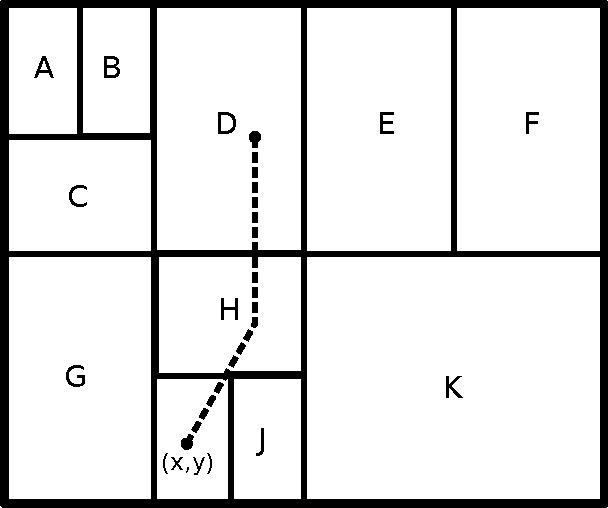
\includegraphics[scale=0.4]{img/algorithms/landmark_binning}
% \caption{Example 2D coordinate overlay and a sample routing path from node D to
% (x,y).}
% \label{fig:landmark_binning}
% \end{figure*}

\emph{Landmark Binning}~\cite{RHMKS2002} partitions close-by nodes 
into bins based on their distance from well known anchor nodes across the
Internet.%, as shown in Figure~\ref{fig:landmark_binning}.
To detect locality, peers mainly use network latency (i.e. \emph{RTT}).
%  as a measurement technique. 
Despite the fact that such delays are not always accurate,
they are used in~\cite{RHMKS2002} for they are 
non-intrusive, transparent and easy to apply.
%%
For the binning to work, a few anchor servers with known
physical locations need to be installed in strategic positions 
across the the Internet. 
It is conjectured~\cite{RHMKS2002} that $12$ such servers can prove
sufficient for the task.
An arriving node measures its distance from these landmarks
and unilaterally decides to join a specific bin based on its measurements.
Specifically, the node measures its round-trip time to each of the landmarks and
orders the resulting \emph{RTT}-values in a decreasing order. 
%%AD I do not understand what the following sentence says..
%%	for each peer there is a different bin right? 
The ordering represents a \emph{bin},
in the sense of close-by nodes having the same landmark ordering and hence
belong to the same bin. 
%%
%%AD I think the above sentence is the main information related in this 
%%   piece of description so it requires a bit better description...
Should there $m$ landmarks be adopted, potentially $m!$  different bins exist.
% This means that a landmark system consisting of $m$ such
% nodes results in $m!$ potential different bins.
%%
The operation of the method is independent of the model 
incorporated by the overlay network and thus it can be
applied with no significant changes to 
both structured and unstructured \p\ systems. 
% \cite{RHMKS2002} has the detailed description of the algorithm for
% both architectures. %%AD obviously!!!!
%%
%%AD why is it important to say this about CDNs???
% Landmark binning is also considered as a good candidate for
% content distribution networks. 
The main disadvantage of the approach is that 
landmark servers must be installed and maintained throughout the world.
Provided that a \p-system often may have a few million nodes 
connected at any given point in time, landmark servers do 
inherently play a pivotal role in the operation of the network.
%%AD rephrased what is below as above...
% A typical P2P network usually has a couple of
% million nodes connected at any given time, thus rendering landmark servers an
% important parameter when designing for large scales.  
%%%%%%%%%%%%%%%%%%
%%AD rephrased what is below as above...
Although latency estimation does not drain network resources,
the scale of the approach does call for an alternative design.
In this respect, \cite{RHMKS2002} advocates the replacement of 
each landmark server by a cluster of servers.
However, this approach may not entirely avoid the creation of 
excessive network traffic flow through its landmark server-clusters.
%%AD rephrased what is below as above...
% The authors claim that
% latency estimation does not drain much from the network resources but in case
% scalability problems arise, they claim the solution is replacing single landmark
% servers with clusters of servers within the same physical area. However, this
% approach does not reduce the possibility of excessive network traffic flow
% through these landmark servers. One other possible problem is the incorrect
% binning caused by the use of inaccurate methods for delay measurement
% (latency is not proven to be a safe way to estimate distance).
%%%%%%%%%%%%%%%%%%%%%%%%%%%%%%%%%%%%%%%%%%%%
%
%
%%
%The algorithm can be considered scalable, as nodes need only compute distances
% to a small number of predefined nodes and thus without exchanging any
%information.
%To answer the question as to whether the algorithm actually contributes
% positively to the construction of an enhanced overlay, the paper defines the
%\emph{gain ratio} as the factor by which the latency reduces when someone
%communicates with a random node from the same bin than with one not in the bin.
%This is implemented with an inter-bin to an intra-bin latency ratio.
%
% TODO: LANDMARK BINNING FOR UNSTRUCTURED OVERLAYS
%
%For unstructured overlays the paper assumes \emph{a set of $n$ nodes where each
% node picks any $k$ neighbor nodes so that the average routing latency on the
%resultant overlay is low (assuming shortest path routing)}. According to the
%proposed heuristic algorithm called \emph{BinShort-Long}, a node picks its
%neighbors by choosing its $\frac{k}{2}$ closest\footnote{If the node's bin is
%not large enough for it to pick these $\frac{k}{2}$ neighbors, it picks the
%required nodes from the bin that matches the most in terms of landmark
%ordering.} ones (named \emph{short links}), using the \emph{binning} scheme and
%the rest $\frac{k}{2}$ randomly (\emph{long links}). The former set produces
%well-connected \emph{pockets} of nearby nodes while the later preserves the
%connectivity of the graph, both yielding a proximity factor of $\alpha = 0.5$
%in an attempt to preserve the beneficial properties of unstructured
%topologies\cite{merugu_str2unstr_2003}.
%
% TODO: SOME DISCUSSION
%
%A potential bottleneck could be the extra load that this
%``ping''-like scheme imposes to the landmarks, especially when we need instant
%reaction from our topology when dealing with the dynamic nature of the p2p
%networks.
%
%One disadvantage of this landmark scheme is related to the additional burden
% imposed to the landmark sites. The authors claim though that the algorithm
%requires so little work by the landmarks (maybe just echo to ping messages)
%that could in effect, act as ``unsuspecting participants''. Even if this is the
%case, the fact that it is not fully distributed, renders the protocol's
%scalability directly vulnerable to any system size increase as well as
%suitable for highly dynamic networks such as ad-hoc networks. Moreover, fixed
%points in a network are inherently more exposed to malicious attacks. The most
%significant downside of the algorithm though is that it can lead to an
%extremely uneven overlay ID distribution causing load unbalances and hot spots.
%Lastly, the scheme is coarse grained when it comes to distinguishing relatively
%close nodes\footnote{In the worst case, all nodes could ve clustered into a
%single bin.}.
%
%%
The landmark binning behaves as follows:
\begin{center}
{\footnotesize
\begin{tabular}{ccc}
\emph{Efficiency} & \emph{Overhead} & \emph{Scalability} \\
\hline
% The technique is coarse grained thus doesn't achieve optimal results
% (especially in small networks)
medium &
% The overhead is confined to the communication of a node with, most probably,
% 12 landmark servers at most.
low &
% The introduction of landmark servers renders the approach not fully
% decentralized, thus preventing it from scaling smoothly. Communicating
% and overloading landmark servers in high-churn systems is another scalability
% concern.
low
\end{tabular}
}
\end{center}

%%%%%%%%%%%%%%%%%%%%%%%%%%%%%%%%%%%%%%%%%%%%%%%%%%%%%%%%%%%%%%%%%%%%%%%%%%%%%%%%
% \subsubsection{mOverlay}
The \emph{mOverlay} approach addresses scalability issues
that might be arise when static landmark servers are in use. 
To this end, the use of dynamic landmarks is proposed.
% \emph{mOverlay} \cite{ZZZSZ2004} tries to 
% addresses the scalability issues that
% might be imposed on networks (i.e. load unbalance) when using static landmark
% servers by introducing dynamic landmarks. 
\emph{mOverlay}'s founding notion is that of a \emph{group} that 
designates a set of peers found in close proximity.
This proximity is user-defined in the protocol and 
may involve metrics including \emph{RTT}s and network latencies.
%%AD rephrased what is below as above... 
% Zhang et al. introduce the notion of a
% \emph{group} which is a set of peers considered close to each other with respect
% to any position in the underlying network, where proximity is defined by some
% user-defined cost metric like RTT, latency or something else. 
%%%%%%%%%%%%%%%%%%%%%%%
By and large a clustering approach, \emph{mOverlay} seeks to 
recreate small-world-like properties by producing a 
two-level hierarchical structure:
at the top level, there are only connections among groups 
while at the bottom, only \emph{intra-group} connections occur among peers.
%%AD rephrased what is below as above... 
% mOverlay is considered a clustering approach since 
% it tries to recreate small-world-like
% properties to the overlay network by creating a two-level hierarchical
% structure, where on the top level we have connections between groups while on
% the bottom we have connections between peers inside groups. 
%%%%%%%%%%%%%%%%%%%%%%%
Clearly, identifying groups and accurately finding the closest group 
to a peer is a fundamental concern in the creation of the overlay.
% Finding the correct closest group is the most important part 
% of the overlay construction. 
Nodes are grouped based on their distance to 
the groups already in the network, rendering
the latter be the \emph{dynamic landmarks} in the process. 
%%AD how do you identify the initial groups????
%%
It is shown that in the proposed scheme, a new peer can 
reach its group by expending at most $O(logN)$ messages
within the network. 
Finally, \emph{mOverlay} maintains stability and constant 
overheads when a host either fails or departs the network;
this is achieved through periodic cache updates and group 
leader selections, should one either leaves or dies.
%%AD rephrased what is below as above...
% The authors formally prove
% that any new node can reach its group by exchanging at most $O(logN)$ messages
% within the network. Finally mOverlay also considers a second important function
% in its protocol which is the constant maintenance of the overlay.
%%%%%%%%%%%%%%%%%%%%%%%%%%%%%%%%%%%%%%%%%%
%%
%
%\paragraph{Locating process} A new coming host, $Q$, first connects to a
%globally known host cache called the \emph{rendezvous point (RP)} in order to
%retrieve the starting point in the overlay, say $A$ in group $1$. Host $Q$
%then, measures its distance to host $A$. At the same time, the later, sends
%information about the neighbor groups of group $1$ back to host $Q$. This list
%is called \emph{candidate group list}, and the new coming host sequentially
%measures its distance to each of them in seek for the closest one. If the
%\emph{grouping criterion} is met, host $Q$ belongs to group $1$. If not, a boot
%host from the closest group is found and the algorithm is re-run until the
%criterion is met or after a predefined number of repetitions. In the later
%case, $Q$ creates a new group comprising itself only. The above protocol does
%not favor hot-spots as it spreads the probability of visiting a group across
%the whole overlay and limits the overhead in the level of $O \left ( log N
%\right )$.
%
%\paragraph{General overlay operations} A set of additional protocols, are also
% introduced, similar to those found in traditional unstructured networks, but
%modified focusing on scalability and robustness. For example a protocol for
%\emph{group formation} is introduced that exploits the inherent characteristic
%of proximity, in the overlay, in order to efficiently detect the neighboring
%groups of a newly formed group from the set of adjacent groups of its closest
%neighbor. Additionally, during \emph{group joining} the corresponding protocol
%denotes the exchange of important information for group maintenance. This can
%be further improved by \emph{information sharing} between nodes of the same
%group, functionality handled by a dedicated flood-like protocol\footnote{Since
%nodes that belong to the same group are physically close this can be achieved
%at a minimum price.}. Moreover, another set of distributed protocols handle the
%\emph{information update}. The information that needs update, in the proposed
%architecture, is
%\begin{inparaenum}[\itshape i\upshape)]
%  \item the host cache, when a new node joins, and
%  \item the neighbors of groups, when a close-by group is generated.
%\end{inparaenum}
%Finally, in case of \emph{host failure} or \emph{host departure} the system is
% able to maintain its stability since there are defined operations for
%periodical host cache update and group leader selection if one leaves or dies.
%
%%
In terms of the stated criteria, \emph{mOverlay} fares as follows:
\begin{center}
{\footnotesize
\begin{tabular}{ccc}
\emph{Efficiency} & \emph{Overhead} & \emph{Scalability} \\
\hline
% The technique is coarse grained thus doesn't achieve optimal results
% (especially in small networks)
medium &
% The algorithm is iterative through the available groups. At each group
% probing of a candidate list must be performed. This process is done at
% bootstrapping time so the overhead increases in high-churn systems
medium &
% The introduction of dynamic landmark servers renders this approach much more
% scalable than the traditional static landmarking techniques 
medium
\end{tabular}
}
\end{center}

%%%%%%%%%%%%%%%%%%%%%%%%%%%%%%%%%%%%%%%%%%%%%%%%%%%%%%%%%%%%%%%%%%%%%%%%%%%%%%%%
%%%%%%%%%%%%%%%%%%%%%%%%%%%%%%%%%%%%%%%%%%%%%%%%%%%%%%%%%%%%%%%%%%%%%%%%%%%%%%%%
\subsection{Discussion on the Algorithms for Unstructured Architectures}
%%%%%%%%%%%%%%%%%%%%%%%%%%%%%%%%%%%%%%%%%%%%%%%%%%%%%%%%%%%%%%%%%%%%%%%%%%%%%%%%
%%%%%%%%%%%%%%%%%%%%%%%%%%%%%%%%%%%%%%%%%%%%%%%%%%%%%%%%%%%%%%%%%%%%%%%%%%%%%%%%

% The introduction of landmark servers renders the approach not fully
% decentralized, thus preventing it from scaling smoothly. Communicating
% and overloading landmark servers in high-churn systems is another scalability
% concern.

While surveying efforts to overcome the mismatch problem
in the area of unstructured \p\ systems,
we came to identify four key methodologies 
utilized by the discussed approaches; these methodologies are:
%%AD shorten below as above...
% In this section, we introduced the topology mismatching problem from the
% perspective of unstructured P2P systems and we visited a series
% of algorithms that have been proposed in the literature to tackle its negative
% influence on performance. In surveying the above algorithms, we identify
% four main methodologies that are used either selectively or in combination
% by each algorithm.  
% These methodologies are:
%%%%%%%%%%%%%%%%%%%%%%%%%%%%
\begin{enumerate}[\itshape i\upshape)]
  \item topology adaptation
  \item forwarding optimization
  \item caching and replication, and
  \item landmarking
\end{enumerate}
Each surveyed approach uses either one or more of the
aforementioned four methodologies. 
Below, we discuss how the proposed protocols use 
elements of the four methodologies and we offer 
a summary qualitative comparison for all surveyed approaches 
applicable for \emph{unstructured} \p \emph{systems}.
%%


%%%%%%%%%%%%%%%%%%%%%%%%%%%%%%%%%%%%%%%%%%%%%%%%%%%%%%%%%%%%%%%%%%%%%%%%%%%%%%%%
\subsubsection{Topology Adaptation Methodology}

Protocols based on topology adaptation 
modify the topology of the \p\ network
using various techniques. 
The two most commonly used approaches to 
topology adaptation are creating
\emph{spanning tree}s using connection graphs 
and creating \emph{clusters} of physically close nodes.

\emph{Narada} and subsequent algorithms including 
\emph{AOTO, LTM, SBO}, try to solve the problem
by building a richer connected graph and forming 
minimum spanning trees over
this graph that can efficiently route messages among peers. 
Even though spanning trees provide efficient query performance, 
their maintenance costs have proven to be a significant limitation. 
This is why the original \emph{Narada} proposal
focused on small groups and thus, is not scalable.  
%%
The \emph{AOTO, LTM} and \emph{SBO} try to 
% Algorithms like AOTO, LTM or SBO try to %%AD this "like" is colloquial 
					  %%   try to avoid it if you can!
overcome these obstacles with 
ingeneous schemes
% clever tricks %%AD this is a bit colloquial
that entail forming minimum spanning trees
for the $2$-hop neighbors ($N^2$) for each node, 
%%AD u imply each has N neighbors above right???
partitioning the graph into two
random groups where each group is responsible for different tasks, 
or performing local optimizations dynamically on the overlay graph. 
%%AD what are these "optimizations" (in 2-3 words  - in sentence)
The advantage of building minimum spanning trees is that 
they maintain the connectivity on the network in
an efficient manner while still preserving the overall search scope. 
However, their construction and the update costs, 
especially in dynamic, high-churn environments, 
causes large additional traffic overhead on the underlying
network~\cite{CRZ2000,CRSZ2001,CRSZ2002}.

%%
%%AD this figure HAS to be referenced in the text!!! 
%%   ALSO - is this ANY different from Fig 4 of the paper??? 
%%   WHY this Fig is being repeated here??? Grand Mystery!!!!
%%	Perhaps we should put one fig similar but more sexy??? ;-)
\begin{figure}[ht]
\centering
\subfigure[Inefficient overlay topology.] {
  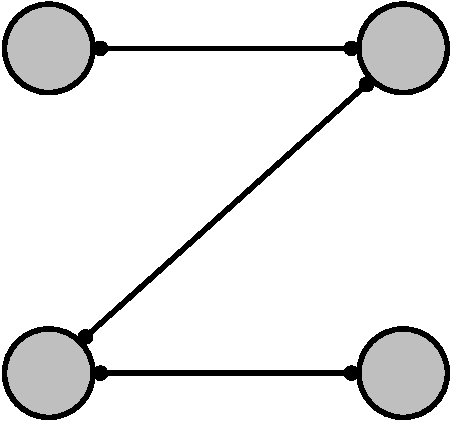
\includegraphics[scale=0.3]{img/pdf/topology-adaptation-before.pdf}
  \label{figure:topology-adaptation:before}
}\qquad\qquad
\subfigure[Efficient overlay topology after adaptation.] {
  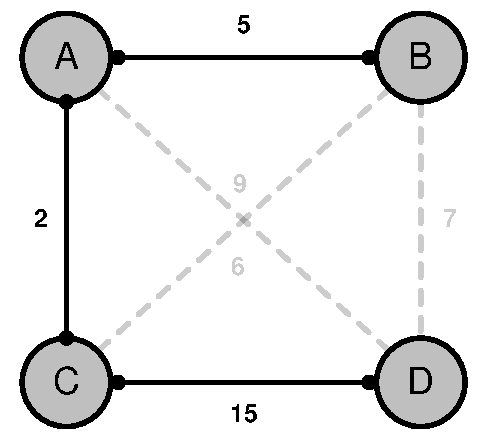
\includegraphics[scale=0.3]{img/pdf/topology-adaptation-after.pdf}
  \label{figure:topology-adaptation:after}
}
\caption{A simplified example on how overlay topology adaptation may improve matters.}
% A simple example of how an overlay topology can be adapted.}
\label{figure:topology-adaptation}
\end{figure}
%%

The cluster-based approaches, on the other hand, 
link physically-close nodes to each other. 
\emph{T2MC}, for example, uses trace-route logs and 
\emph{DDNO} exploits domain names to cluster nodes in proximity. 
Unfortunately, commonly used
methods for proximity detection across Internet do not always return
reliable results and therefore, mapping accuracy is not guaranteed. 
Moreover, trace-route is a computing resource ``heavy-weigth'' utility 
and so  a number of network equipment vendors do not allow
trace-route calls at all. %%AD do you have a refeerence or two in here???
%%
The most problematic aspect of clustering, though, is
its nature per se. 
Limited connectivity among the various local domains can
significantly shrink the search scope, negatively affecting the query response
time that the \p\ user experiences. 
% Techniques, like DDNO, that try to 
Among others, \emph{DDNO} tries to 
balance the efficiency of the clustering approach 
with enhanced node connectivity. 
In particular, \emph{DDNO} attemps to address this limitation
by forcing half of each node's connections to be with other, randomly
selected, nodes in the network.
%%AD you mean the "logical network"? the p2p network???

As a methodology, 
topology adaptation ultimately aims to reduce the 
average path traversing cost from one node to another.
In doing so, topology adaptation  re-arranges the 
overlay network so that it becomes a better fit 
for the underlying \emph{IP} network
as Figure~\ref{figure:topology-adaptation} depicts.
Despite the fact that the above is a plausible proposition,
it is not always advantageous.
% This is fair in the general case but not always. 
%%
For example, an topology adaptive algorithm can exchange 
a slow edge in the overlay with a faster one
thus reducing the average latency of the network communication. 
The pitfall here is that this new virtual link 
can traverse a fast \emph{AS}--to--\emph{AS} 	
			%%AD you mean Autonomous Systems here?? 
		  	%%    What is this AS???
link meaning that even though message
round-trip-time is reduced, it has more cost 
in terms of communication network economics and management.
%%AD just check the above sentence for correctness..


% These approaches include creating spanning trees using
%connection graphs, creating cluster of physically close nodes, or using latency
%information to detect proximity. The brief description of each category is
%presented below:
%
%  \begin{itemize}
%    \item \emph{Spanning tree based}. These approaches construct of a rich
%    graph  based on the network connections and build minimum spanning tree
%    on the graphs, causing large traffic overhead to the system
%    \cite{chu_esm_2000,chu_esm_2002}.
%
%    \item \emph{Cluster based}. These approaches select to link physically
%    closer nodes with each other, therefore shrink the search scope
%    significantly while mapping accuracy is not always guaranteed.
%
%    \item \emph{Minimum latency first}. Use of latency as a metric to calculate
%    distance among peers. They require global latency information
%    ``landmarks''\footnote{Measuring latency between peers and stable Internet
%    servers.}.
%
%  \end{itemize}

%%%%%%%%%%%%%%%%%%%%%%%%%%%%%%%%%%%%%%%%%%%%%%%%%%%%%%%%%%%%%%%%%%%%%%%%%%%%%%%%
\subsubsection{Forwarding Optimization Methodology}

% Researchers initially started considering alternatives for services who
% implement one-to-many communication schemes, like IP multi-cast, on the
% application layer (i.e. Narada). Application level multi-cast protocols
% are generic protocols that can be applied to both P2P file sharing systems,
% as well as content distribution networks. Application layer multi-cast,
% however,
% is not as efficient as the one enabled by IP and still struggles to ease the
% difficulties imposed by the topology mismatch problem.

%Forwarding optimization can reduce the emitted messages flooding the overlay and
%as a consequence the overall burden, network resources have to handle. In the
%first realization of the Gnutella protocol, each query request received by a
%peer, was then forwarded to all of its neighbors. This was the source of
%unnecessary, sometimes redundant traffic. 


%%AD I think you will need to sprinkle some references of those surveyed 
%%	in this subsubsection.. As opposed to what done above, 
%%	this subsubsection has no reference in the text!!!!
Approaches based on forwarding-optimization 
propose intelligent forwarding link selection for a message's next
hop across a routing path. 
The selection criteria vary depending on the
algorithm, but they mainly use one or more statistical heuristics. 
These can range from simple and rather obvious ones, 
including the latency of the link between the nodes or
the exposure of specific features such as high processing bandwidth, high
capacity, or low latency, 
to more sophisticated alternatives that may even take
into account application level requirements such as 
the reliability or friendship. 

Figure~\ref{figure:forwarding-optimisation} shows a simple example
of how forwarding optimization may work.
%%
\begin{figure}[ht]
\centering
\subfigure[Typical blind flooding.] {
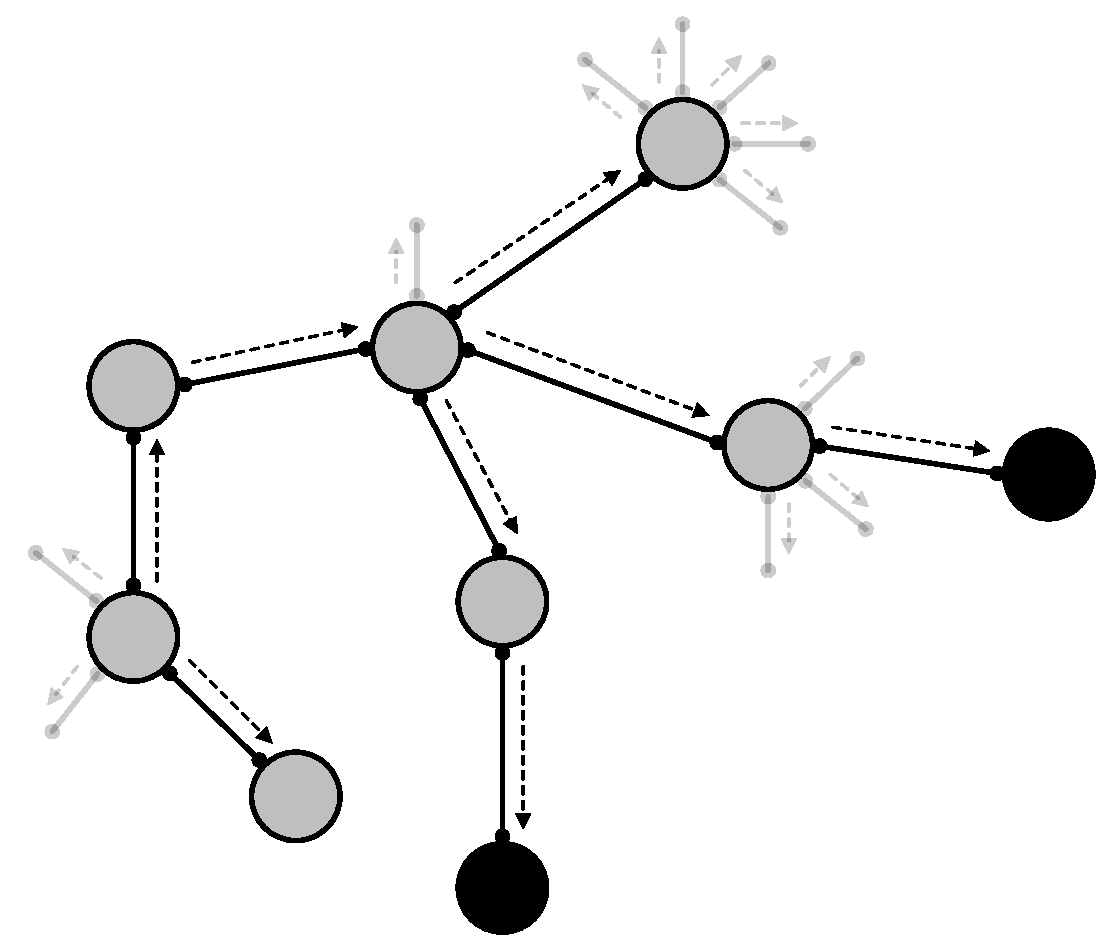
\includegraphics[scale=0.20]{img/pdf/forwarding-optimization-before.pdf}
  \label{figure:forwarding-optimisation:before}
}\qquad\qquad
\subfigure[A node can decide where to forward the messages.] {
  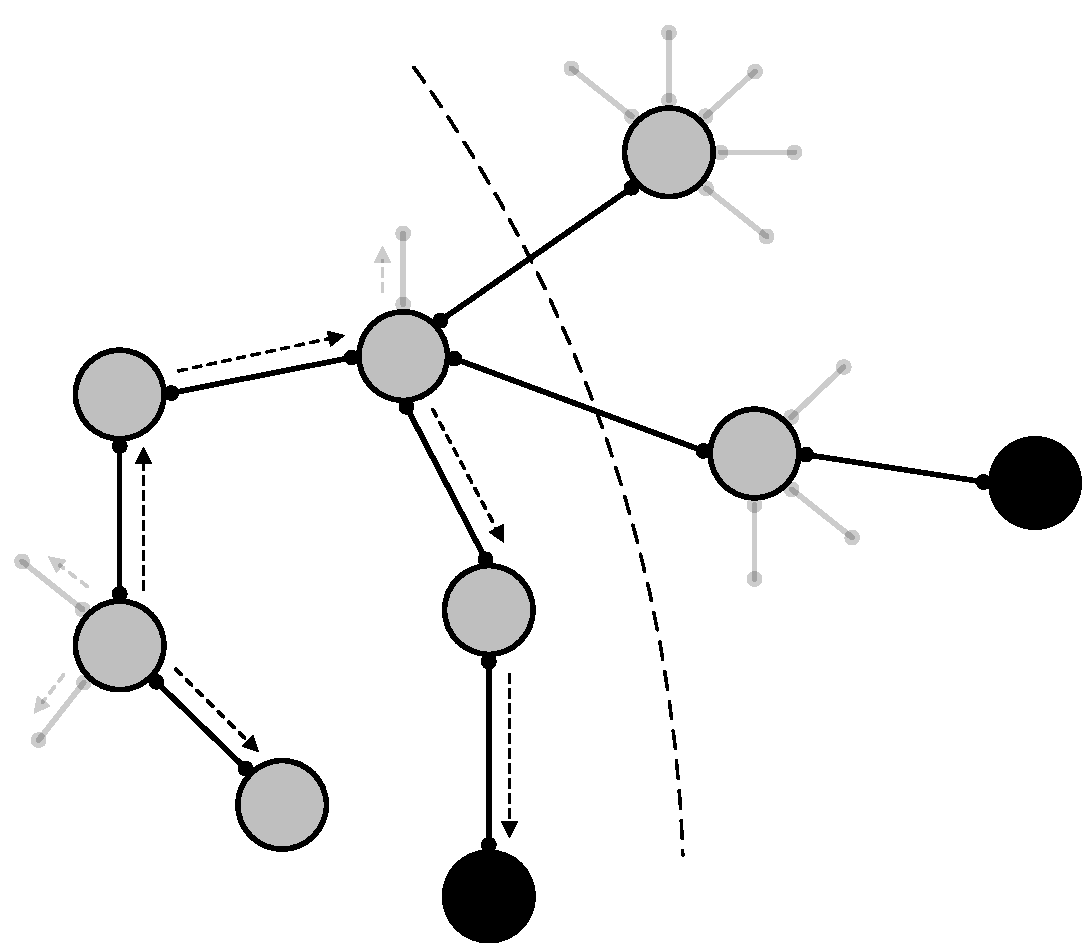
\includegraphics[scale=0.20]{img/pdf/forwarding-optimization-after.pdf}
  \label{figure:forwarding-optimisation:after}
}
\caption{Forwarding optimization in constraining message flooding.}
\label{figure:forwarding-optimisation}
\end{figure}
%%
Fig.~\ref{figure:forwarding-optimisation:before} 
% Sub-figure~\ref{figure:forwarding-optimisation:before} 
shows a protocol that simply floods the entire network 
in search of object found in the nodes colored in black.
% for search of an object the existence of which is
% denoted by black nodes. 
Alternatively, a node can decide to forward its
messages not to every output link but to a specific 
or subset of its outgoing links. 
In Sub-figure~\ref{figure:forwarding-optimisation:after}, the node in the
In Fig.~\ref{figure:forwarding-optimisation:after}, 
the node in the middle, does not flood its neighbors as instead 
in only picks one of them.
The dashed line on the right, shows that, 
for this routing process, the protocol has
rendered two potential forwarding paths as inefficient (e.g., the target nodes
show overloading signs). 
On one hand, forward
optimisation approaches have 
the advantage of enhancing the
search responsiveness and reducing the aggregate resource 
usage of the physical network. On the other, 
they suffer from drastic reduction of the search
scope (in Fig.~\ref{figure:forwarding-optimisation:after} the object on
the far right is not reached) thus limiting the scalability of the whole
network. 
Moreover, they adress the problem of the mismatch in a limited manner
% do not actually address the problem of topology mismatch
since they do not provide any guarantees 
that overlay and underlying topologies are
aligned with each other let alone quantify the mismatch 
and try to alleviate.
% Like all other methodologies, 
Forwarding based optimisations are commonly applied in
conjunction with other methodologies to improve 
the quality of the \p\ systems.


%Expanding the search scope, on the other hand, is no easy task
%because the overhead of forming multi-cast trees is proportional to the
%multi-cast group size.
%forwarding based schemes do not consider dynamic joining
%and leaving of peers so they do not scale well on dynamic environments.


%%%%%%%%%%%%%%%%%%%%%%%%%%%%%%%%%%%%%%%%%%%%%%%%%%%%%%%%%%%%%%%%%%%%%%%%%%%%%%%%
\subsubsection{Caching and Replication Methodology}

%%AD in this portion there is NOT much about replication... 
%%	ALSO, references to surveyed works as missing.. (other than
%%	KAzaa!) -  Sprinkle some around the text...
Caching is widely used to exploit locality and minimize redundant
transfer of data. Caching has with much success been successfully 
adopted by web and file server application environments. 
Since peers in a \p\ system also operate as servers,
it is intuitively expected that \p\ file sharing systems can also benefit from
caching in improving performance and reducing overall resource usage. 
However, the design of caches in this context 
is non-trivial compared to the web-based caching. 
Due to the fact nodes play the double role of server and client,
two important issues have to be considered at design time. 
First, the lifetime of a query is short, as the nodes join 
and leave frequently. Second, the result
of a single query string is not always the same, as this depends on the
source of the query, the \emph{TTL} value set for the messages, 
the current interconnection of peers and the 
high volatility of the environment. 
Thus, to develop a successful caching system for a \p\ architecture, these
parameters also have to be carefully considered. 
\p\ caching/replication can be applied
at two different levels, namely caching indices or pointers to data 
(Fig.~\ref{figure:replication:index}) or caching the data itself 
(Fig.~\ref{figure:replication:data}). 
%%%
\begin{figure}[ht]
\centering
\subfigure[Indexing can reduce the cost of the last hop.] {
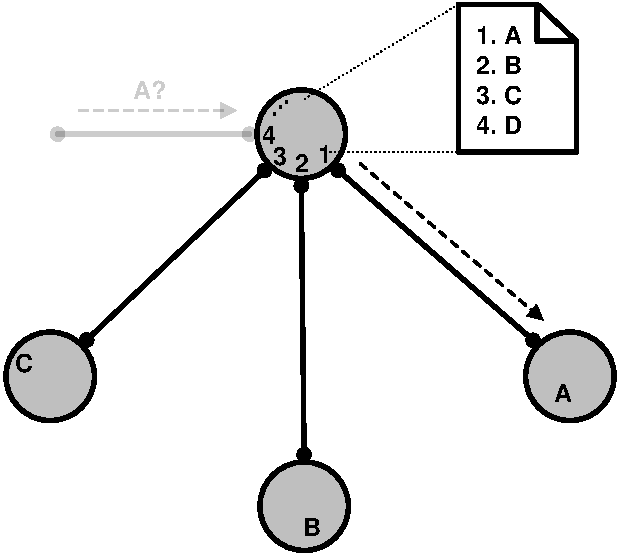
\includegraphics[scale=0.3]{img/pdf/replication-index.pdf}
  \label{figure:replication:index}
}\qquad\qquad
\subfigure[Data replication along the path of a successful query.] {
  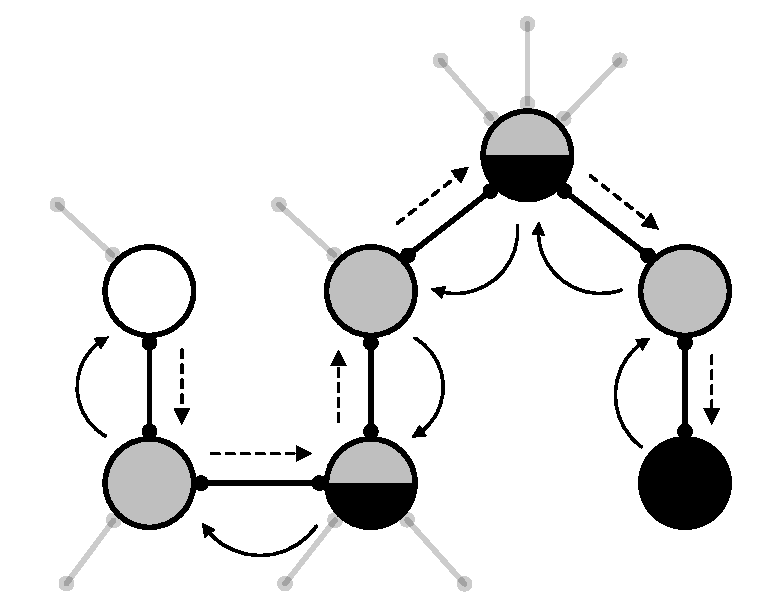
\includegraphics[scale=0.3]{img/pdf/replication-data.pdf}
  \label{figure:replication:data}
}
\caption{Index and data replication strategies.}
\label{figure:replication}
\end{figure}
%%
Successful implementations have
already been developed in some commercial \p\ systems, like 
\emph{KaZaA}, which uses
caching of indices on its super-peer level. 
%%%
Even though the state of the art in \p\ protocols using caching methods
helps reduce the burden of network resources, 
their contribution in addressing the mismatch problem 
remains limited.
%%AD I am not sure what the following piece says....
%%	tried to rephrase as above...
% Unfortunately, even though the state of the art 
% in \p\ protocols using caching methods reduce the resource
% usage of the network, 
% they also fail to consistently address typical problems
% of a topologically mismatched environment such as duplication of messages.
%%%%%%%%%%%%%%%%%%%%%%% 

%\subsection{Cache Based}
%
%Caching based protocols are effectively used to reduce traffic costs and
%response
%times. The caching policy varies depending on the way protocol handles the
%index and the
%content. Centralized P2P systems
%use central index servers, while local caching systems, such as KazaA, use
%super peers
%to cache indices in a distributed way. Content caching is also possible in P2P
%systems, where nodes cache the forwarded content for further retrievals.
%Although caching has the above mentioned advantages,  duplication
%of messages still exist, which limits the scalability of these approaches.
%Therefore, cache based approaches are analyzed in the following categories:
%  \begin{itemize}
%    \item \emph{data index caching},
%    \item \emph{content index caching},
%    \item \emph{centralized}, and
%    \item \emph{local}.
%  \end{itemize}

%%%%%%%%%%%%%%%%%%%%%%%%%%%%%%%%%%%%%%%%%%%%%%%%%%%%%%%%%%%%%%%%%%%%%%%%%%%%%%%%
\subsubsection{Landmarking}\label{sec:landmark}

In landmark-based algorithms, nodes use network delay (e.g., \emph{RTT}) as a
distance measurement method to position themselves with respect to ``a priori''
known servers on the Internet. 
These landmark servers are used
by nodes to estimate their positions based on the intuitive assumption that
nodes
with similar distances to a set of landmarks, are physically close to each
other, as well, over the network. 
In Figure~\ref{figure:landmarking} the newly
arriving peer, measures its distance to an array of landmark point denoted as
$Ln$ and and makes a sorted list of the peers, say in increasing order. Then in
order to choose the already participating peers with which to connect to,
compares its list to the list of the potential neighbor. Peers with similar
measured distances to the these landmark points are likely to be close to
each other as well.
%%
\begin{figure}[ht]
\centering
  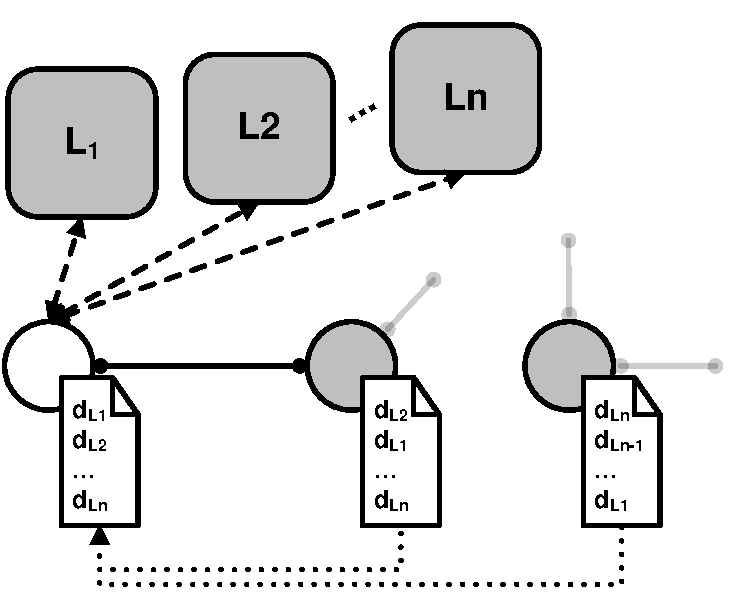
\includegraphics[scale=0.4]{img/pdf/landmarking.pdf}
\caption{Landmark binning during node bootstrap.}
\label{figure:landmarking}
\end{figure}


Landmark based protocols have four important drawbacks: First, the network
delay is not a reliable distance estimation method. For example, based on the
load on the network, the delay to certain nodes or networks can change from time
to time, which will eventually affect the distance measurements and wrong
measurements will lead to wrong estimated positions for the nodes, or incorrect
and non optimal clusterings of the nodes. Second, relying on predefined nodes
make the whole paradigm not fully distributed and the landmark system prone to
become a single point of failure. Third, using
landmark servers requires costly installation and maintenance of landmark
infrastructure across the whole Internet and for all the different autonomous
system domains. 
As popular \p\ file sharing applications usually have millions
of peers connected at any time, the network costs
of maintaining these landmark servers will likely be quite high. 
A possible solution to
the scalability problem of the static landmark servers is to use ordinary nodes
as dynamic landmarks once they estimate their own positions. Even though this
approach scales much better than static landmark servers, the measurement
accuracy problem affects the overall performance of the system. Moreover,it can
be characterized as a rather coarse-grained approximation, therefore not
particularly well suited for detecting the correct positions of nodes within
close distance to each other.
%%AD ok how about ay advantages?? Any referencess??? 
%%	Also, a bit of a discussion is missing on hybrid approaches surveyed
%%	for example which approaches use a combo of these methodologies???

Table~\ref{unstructured:table} offers a summary overview of the algorithms
we saw earlier in this section and for each algorithm, shows which of the
aforementioned methodologies it incorporates, along with its 
highlights and a rough estimation of the
positive and negative aspects of its implementation.

%%%%%%%%%%%%%%%%%%%%%%%%%%%%%%%%%%%%%%%%%%%%%%%%%%%%%%%%%%%%%%%%%%%%%%%%%%%%%%%%
%\renewcommand\arraystretch{1.9}% (MyValue=1.0 is for standard)

\begin{landscape}
%\begin{figure}[h!]
\hspace{-3ex}
\begin{center}
\footnotesize
%\begin{tabular}{
\begin{longtable}{
|m{2cm}
|m{1cm}
|m{1cm}
|m{1cm}
|m{1cm}
|m{3cm}
|m{5cm}
|
}
% |>{\columncolor[gray]{.7}}m{0.1\columnwidth}
% |>{\columncolor[gray]{.9}}m{0.1\columnwidth}
% |>{\columncolor[gray]{.8}}m{0.1\columnwidth}
% |>{\columncolor[gray]{.9}}m{0.1\columnwidth}
% |>{\columncolor[gray]{.9}}m{0.1\columnwidth}
% |>{\columncolor[gray]{.8}}m{0.1\columnwidth}
% |>{\columncolor[gray]{.9}}m{0.1\columnwidth}
% |}
\caption[Summary table for unstructured algorithms]{Summary table for unstructured algorithms.} \label{unstructured:table} \\
\hline
%%%%%%%%%%%%%%%%%%%%%%%%%%%%%%%%%%%%%%%%%%%%%%%%%%%%%%%%%%%%%%%%%%%%%%%%%%%%%%%%
% first head
\rowcolor[gray]{.5}
\textbf{Algorithm / Paper} &
\textbf{Topology Adaptation} &
\textbf{Forwarding Optimization} &
\textbf{Caching / Replication} &
\textbf{Landmarking} &
\textbf{Highlights} &
\textbf{Pros / Cons}\\
\hline
\endfirsthead
%%%%%%%%%%%%%%%%%%%%%%%%%%%%%%%%%%%%%%%%%%%%%%%%%%%%%%%%%%%%%%%%%%%%%%%%%%%%%%%%
% subsequent heads
\multicolumn{7}{c}%
{\tablename\ \thetable\ -- \textit{Continued from previous page}} \\
\hline
\rowcolor[gray]{.5}
\textbf{Algorithm / Paper} &
\textbf{Topology Adaptation} &
\textbf{Forwarding Optimization} &
\textbf{Caching / Replication} &
\textbf{Landmarking} &
\textbf{Highlights} &
\textbf{Pros / Cons}\\
\hline
\endhead
%%%%%%%%%%%%%%%%%%%%%%%%%%%%%%%%%%%%%%%%%%%%%%%%%%%%%%%%%%%%%%%%%%%%%%%%%%%%%%%%
% foot
\hline \multicolumn{7}{r}{\textit{Continued on next page}} \\
\endfoot
%%%%%%%%%%%%%%%%%%%%%%%%%%%%%%%%%%%%%%%%%%%%%%%%%%%%%%%%%%%%%%%%%%%%%%%%%%%%%%%%
% last foot
\hline
\endlastfoot
%%%%%%%%%%%%%%%%%%%%%%%%%%%%%%%%%%%%%%%%%%%%%%%%%%%%%%%%%%%%%%%%%%%%%%%%%%%%%%%%
% data
\textbf{\cite{YG-M2002}} &
{\large \Square} &
{\large \CheckedBox} &
{\large \CheckedBox} &
{\large \Square} &
\begin{tabular}[l]{m{3cm}}
Iterative Deepening (ID).\\
Directed BFS (DBFS).\\
Local Indices (LI).
\end{tabular} &
\begin{tabular}[l]{m{5cm}}
+ ID reduces the messages especially in upper levels of the tree.\\
%+ DBFS ??????\\
+ LI reduces aggregate bandwidth usage and improves query efficiency.\\
-- ID needs evaluation time between iterations.\\
-- DBFS uses heuristics so it depends on their efficient choice.\\
-- LI add index update overhead which might be heavy process especially in high-churn systems.
\end{tabular}
\\
\hline
%%%%%%%%%%%%%%%%%%%%%%%%%%%%%%%%%%%%%%%%%%%%%%%%%%%%%%%%%%%%%%%%%%%%%%%%%%%%%%%%
\textbf{DAPS \cite{ZL2005}} &
{\large \Square} &
{\large \Square} &
{\large \Square} &
{\large \Square} &
\begin{tabular}[l]{m{3cm}}
Clustered routing tables based on delay.\\
Pruning flood, an iterative deepening and multiple BFS approach with a pruning
boundary.
\end{tabular} &
+ It is a system between structured and unstructured.
\\
\hline
%%%%%%%%%%%%%%%%%%%%%%%%%%%%%%%%%%%%%%%%%%%%%%%%%%%%%%%%%%%%%%%%%%%%%%%%%%%%%%%%
\textbf{Gia \cite{CRBLS2003}} &
{\large \CheckedBox} &
{\large \CheckedBox} &
{\large \CheckedBox} &
{\large \Square} &
\begin{tabular}{m{3cm}}
Random Walks (RW).
\end{tabular} &
\begin{tabular}[l]{m{5cm}}
+ RWs issue one copy of the query thus not flooding the whole network.\\
-- RWs can reduce search scope.\\
\end{tabular}
\\
\hline
%%%%%%%%%%%%%%%%%%%%%%%%%%%%%%%%%%%%%%%%%%%%%%%%%%%%%%%%%%%%%%%%%%%%%%%%%%%%%%%%
\textbf{DCMP \cite{ZKB2008}} &
{\large \CheckedBox} &
{\large \Square} &
{\large \Square} &
{\large \Square} &
\begin{tabular}{m{3cm}}
Cycle detection.
\end{tabular} &
\begin{tabular}[l]{m{5cm}}
+ Drastically reduces duplicate messages.\\
-- Cannot detect cycles in distance bigger than the TTL value of the IC message.\\
\end{tabular}
\\
\hline
%%%%%%%%%%%%%%%%%%%%%%%%%%%%%%%%%%%%%%%%%%%%%%%%%%%%%%%%%%%%%%%%%%%%%%%%%%%%%%%%
\textbf{\cite{CS2002}} &
{\large \Square} &
{\large \Square} &
{\large \CheckedBox} &
{\large \Square} &
\begin{tabular}[l]{m{3cm}}
Uniform replication.\\
Proportional replication.\\
Square root replication allocation.
\end{tabular} &
\begin{tabular}[l]{m{5cm}}
+ Uniform replication reduces time spend on unsuccessful searches.\\
+ Reduces search time for frequent queries.\\
-- Proportional replication struggles in locating rare objects.
\end{tabular}
\\
\hline
%%%%%%%%%%%%%%%%%%%%%%%%%%%%%%%%%%%%%%%%%%%%%%%%%%%%%%%%%%%%%%%%%%%%%%%%%%%%%%%%
% \textbf{Tracing a large-scale Peer to Peer System: an hour in the life of Gnutella} &
% ? &
% ? &
% ? &
% ? &
% ? &
% ?
% \\
% \hline
%%%%%%%%%%%%%%%%%%%%%%%%%%%%%%%%%%%%%%%%%%%%%%%%%%%%%%%%%%%%%%%%%%%%%%%%%%%%%%%%
\textbf{Narada \cite{CRZ2000}} &
{\large \Square} &
{\large \CheckedBox} &
{\large \Square} &
{\large \Square} &
\begin{tabular}[l]{m{3cm}}
Mess creation.\\
Minimum spanning trees.
\end{tabular} &
\begin{tabular}[l]{m{5cm}}
+ Mess and trees are kept up to date in high churn environments.\\
-- Works well only for small groups of peers.
\end{tabular}
\\
\hline
%%%%%%%%%%%%%%%%%%%%%%%%%%%%%%%%%%%%%%%%%%%%%%%%%%%%%%%%%%%%%%%%%%%%%%%%%%%%%%%%
\textbf{AOTO \cite{LZXN2003}} &
{\large \CheckedBox} &
{\large \CheckedBox} &
{\large \Square} &
{\large \Square} &
\begin{tabular}[l]{m{3cm}}
Minimum spanning trees.\\
Peer proximity heuristic for removing costly links.
\end{tabular} &
\begin{tabular}[l]{m{5cm}}
+ Spanning trees only to immediate neighbors so no flooding and at the same time
no shrinked search scope.\\
+ Selective flooding effectiveness is detached from physical or overlay topologies.\\
+ The more logical neighbors, the more effective selective flooding becomes\\
-- High recalculation costs.\\
-- No sophisticated selection policy for candidate non-flooding peers.
\end{tabular}
\\
\hline
%%%%%%%%%%%%%%%%%%%%%%%%%%%%%%%%%%%%%%%%%%%%%%%%%%%%%%%%%%%%%%%%%%%%%%%%%%%%%%%%
\textbf{ACE \cite{LZXN2004}} &
{\large \CheckedBox} &
{\large \CheckedBox} &
{\large \Square} &
{\large \Square} &
\begin{tabular}[l]{m{3cm}}
Minimum spanning trees.\\
1-hop proximity heuristic.
\end{tabular} &
\begin{tabular}[l]{m{5cm}}
+ No flooding.\\
+ Less overhead compared to AOTO since computation is done within a certain diameter from the source peer.
-- Slow convergence speed.\\
-- Enhanced topology optimization comes to the expence of higher communication/computation overhead.
\end{tabular}
\\
\hline
%%%%%%%%%%%%%%%%%%%%%%%%%%%%%%%%%%%%%%%%%%%%%%%%%%%%%%%%%%%%%%%%%%%%%%%%%%%%%%%%
\textbf{LTM \cite{LLXNZ2004}} &
{\large \CheckedBox} &
{\large \Square} &
{\large \Square} &
{\large \Square} &
\begin{tabular}[l]{m{3cm}}
TTL detector (2-hop distance).\\
Delayed low productive connection cutting.
\end{tabular} &
\begin{tabular}[l]{m{5cm}}
+ Compared to AOTO, ACE and SBO achieves faster convergence speed.\\
-- Creates more overhead than AOTO, ACE and SBO.\\
-- Needs synchronization of peer clocks.\\
-- Does not consider shortcuts created by powerful peers when choosing to disable connections (only uses delay metric).
\end{tabular}
\\
\hline
%%%%%%%%%%%%%%%%%%%%%%%%%%%%%%%%%%%%%%%%%%%%%%%%%%%%%%%%%%%%%%%%%%%%%%%%%%%%%%%%
\textbf{SBO \cite{LXN2004}} &
{\large \CheckedBox} &
{\large \CheckedBox} &
{\large \Square} &
{\large \Square} &
\begin{tabular}{m{3cm}}
Red/white bipartite overlay.
\end{tabular} &
\begin{tabular}[l]{m{5cm}}
+ Efficient in both static and dynamic environments.\\
+ Compared to AOTO incurs half the overhead.\\
-- Needs almost double the steps of LTM to converge (static or dynamic environments).
\end{tabular}
\\
\hline
%%%%%%%%%%%%%%%%%%%%%%%%%%%%%%%%%%%%%%%%%%%%%%%%%%%%%%%%%%%%%%%%%%%%%%%%%%%%%%%%
\textbf{THANCS \cite{LNXE2005}} &
{\large \CheckedBox} &
{\large \CheckedBox} &
{\large \Square} &
{\large \Square} &
\begin{tabular}[l]{m{3cm}}
Local optimum heuristic\\
Piggybacking neighbor distance in queries
\end{tabular} &
\begin{tabular}[l]{m{5cm}}
+ Completely distributed approach.\\
+ Presents trivial overhead compared to the query cost savings.\\
+ Convergent speed faster among AOTO, LTM, SBO.\\
+ Does not shrink the search scope.\\
-- Design cannot be extended to support non-flooding-based systems.
\end{tabular}
\\
\hline
%%%%%%%%%%%%%%%%%%%%%%%%%%%%%%%%%%%%%%%%%%%%%%%%%%%%%%%%%%%%%%%%%%%%%%%%%%%%%%%%
\textbf{HAND \cite{CLZHC2006}} &
{\large \CheckedBox} &
{\large \Square} &
{\large \Square} &
{\large \Square} &
\begin{tabular}{m{3cm}}
Triple-hop adjustment.
\end{tabular} &
\begin{tabular}[l]{m{5cm}}
+ No need for clock sync.\\
+ Fully distributed.\\
+ Low overhead for the triple hop adjustment.\\
+ Applicable to both static and dynamic environments.\\
+ Low query response time.\\
-- Compared to LTM has lower traffic reduction and query response rates.
\end{tabular}
\\
\hline
%%%%%%%%%%%%%%%%%%%%%%%%%%%%%%%%%%%%%%%%%%%%%%%%%%%%%%%%%%%%%%%%%%%%%%%%%%%%%%%%
\textbf{APS \cite{BFLZ2003}} &
{\large \CheckedBox} &
{\large \Square} &
{\large \Square} &
{\large \Square} &
\begin{tabular}{m{3cm}}
machine learning adaptive mechanism.
\end{tabular} &
\begin{tabular}[l]{m{5cm}}
+ Fully dynamic switching decision policy.\\
- Low convergence due to the learning process.
\end{tabular}
\\
\hline
%%%%%%%%%%%%%%%%%%%%%%%%%%%%%%%%%%%%%%%%%%%%%%%%%%%%%%%%%%%%%%%%%%%%%%%%%%%%%%%%
\textbf{ITA \cite{PRFM2009}} &
{\large \CheckedBox} &
{\large \CheckedBox} &
{\large \Square} &
{\large \Square} &
\begin{tabular}[l]{m{3cm}}
Short/long connections.\\
Local flooding.
\end{tabular} &
\begin{tabular}[l]{m{5cm}}
+ Low clustering.\\
+ Large peer coverage.\\
+ Reduced duplication.\\
+ Low or no impact to other mechanisms of unstructured p2p networks (e.g. 1-hop
replication, dynamic querying).
\end{tabular}
\\
\hline
%%%%%%%%%%%%%%%%%%%%%%%%%%%%%%%%%%%%%%%%%%%%%%%%%%%%%%%%%%%%%%%%%%%%%%%%%%%%%%%%
\textbf{EGOIST \cite{SLLBBR2008}} &
{\large \CheckedBox} &
{\large \Square} &
{\large \Square} &
{\large \Square} &
\begin{tabular}{m{3cm}}
Selfish shortest path routing
\end{tabular} &
\begin{tabular}{m{3cm}}
-- constructs a global view of the network
\end{tabular}
\\
\hline
%%%%%%%%%%%%%%%%%%%%%%%%%%%%%%%%%%%%%%%%%%%%%%%%%%%%%%%%%%%%%%%%%%%%%%%%%%%%%%%%
\textbf{BNS \cite{BCCMSBZ2006}} &
{\large \CheckedBox} &
{\large \Square} &
{\large \CheckedBox} &
{\large \Square} &
\begin{tabular}[l]{m{3cm}}
ISP clustering (tracker-side or ISP-side detection).\\
Bandwidth throttling.\\
Caching.
\end{tabular} &
\begin{tabular}[l]{m{5cm}}
+ Localizes traffic within an ISP.\\
+ Preserves the efficiency of BitTorrent protocol.\\
-- Needs ISPs to either provide information or infrastructure changes.\\
-- Locality-based approaches do not treat fair all peers.
\end{tabular}
\\
\hline
%%%%%%%%%%%%%%%%%%%%%%%%%%%%%%%%%%%%%%%%%%%%%%%%%%%%%%%%%%%%%%%%%%%%%%%%%%%%%%%%
\textbf{Ono \cite{CB2008}} &
{\large \CheckedBox} &
{\large \Square} &
{\large \Square} &
{\large \CheckedBox} &
\begin{tabular}[l]{m{3cm}}
ISP clustering.\\
Landmarking based on existing CDN infrastructure (CDN redirection measurements).
\end{tabular} &
\begin{tabular}[l]{m{5cm}}
+ Needs no ISP cooperation.\\
+ Needs no extra infrastructure.\\
+ Needs no network topology information.\\
-- Locality based approaches do not treat fair all peers.
\end{tabular}
\\
\hline
%%%%%%%%%%%%%%%%%%%%%%%%%%%%%%%%%%%%%%%%%%%%%%%%%%%%%%%%%%%%%%%%%%%%%%%%%%%%%%%%
\textbf{\cite{LCLX2009}} &
{\large \CheckedBox} &
{\large \Square} &
{\large \Square} &
{\large \Square} &
\begin{tabular}{m{3cm}}
AS hop count minimization on neighbor selection, on chocking/unchocking
mechanisms and on next-chunk picking.
\end{tabular} &
\begin{tabular}[l]{m{5cm}}
+ Optimization of the inter-AS traffic.\\
-- Locality based approaches do not treat fair all peers.
\end{tabular}
\\
\hline
%%%%%%%%%%%%%%%%%%%%%%%%%%%%%%%%%%%%%%%%%%%%%%%%%%%%%%%%%%%%%%%%%%%%%%%%%%%%%%%%
\textbf{TopBT \cite{RTLCGZ2010}} &
{\large \CheckedBox} &
{\large \Square} &
{\large \Square} &
{\large \Square} &
\begin{tabular}[l]{m{3cm}}
Peer selection metric that takes both downloading speed and network topology
into account.\\
Applied in multiple places of the BitTorrent protocol (bootstrap, connection
establishment/replacement, unchocking).
\end{tabular} &
\begin{tabular}[l]{m{5cm}}
+ No need for additional infrastructure.\\
+ Enhances both traffic and downloading.\\
-- Needs off-line processing of BGP dumps.
\end{tabular}
\\
\hline
%%%%%%%%%%%%%%%%%%%%%%%%%%%%%%%%%%%%%%%%%%%%%%%%%%%%%%%%%%%%%%%%%%%%%%%%%%%%%%%%
\textbf{UTAPS \cite{LCY2008}} &
{\large \CheckedBox} &
{\large \Square} &
{\large \Square} &
{\large \CheckedBox} &
\begin{tabular}{m{3cm}}
Network tomography to construct a picture for the underlying network.
\end{tabular} &
\begin{tabular}[l]{m{5cm}}
+ Reduced ISP burden.\\
+ Better downloading speeds.\\
-- Small, laboratory-scale evaluation setup.
\end{tabular}
\\
\hline
%%%%%%%%%%%%%%%%%%%%%%%%%%%%%%%%%%%%%%%%%%%%%%%%%%%%%%%%%%%%%%%%%%%%%%%%%%%%%%%%
\textbf{\cite{QLZG2009}} &
{\large \CheckedBox} &
{\large \Square} &
{\large \Square} &
{\large \CheckedBox} &
\begin{tabular}{m{3cm}}
Cluster peers in a swarm into local, intra- and inter-ISP.
\end{tabular} &
\begin{tabular}[l]{m{5cm}}
+ Reduced ISP burden.\\
+ Better downloading speeds.\\
-- Similarly to UTAPS, the evaluation setup was small scale.
\end{tabular}
\\
\hline
%%%%%%%%%%%%%%%%%%%%%%%%%%%%%%%%%%%%%%%%%%%%%%%%%%%%%%%%%%%%%%%%%%%%%%%%%%%%%%%%
\textbf{PROP \cite{QCYCZ2007}} &
{\large \CheckedBox} &
{\large \Square} &
{\large \Square} &
{\large \Square} &
\begin{tabular}{m{3cm}}
Neighbor exchange between peers.
\end{tabular} &
\begin{tabular}[l]{m{5cm}}
+ Cooperation between peers.\\
+ Guarantees the connectivity of the network between exchanges.\\
\end{tabular}
\\
\hline
%%%%%%%%%%%%%%%%%%%%%%%%%%%%%%%%%%%%%%%%%%%%%%%%%%%%%%%%%%%%%%%%%%%%%%%%%%%%%%%%
% \textbf{Resolving the Topology Mismatch Problem in Unstructured Peer-to-Peer Networks} &
% ? &
% ? &
% ? &
% ? &
% ? &
% ?
% \\
% \hline
%%%%%%%%%%%%%%%%%%%%%%%%%%%%%%%%%%%%%%%%%%%%%%%%%%%%%%%%%%%%%%%%%%%%%%%%%%%%%%%%
\textbf{DDNO \cite{Z-YK2005}} &
{\large \CheckedBox} &
{\large \Square} &
{\large \Square} &
{\large \Square} &
\begin{tabular}{m{3cm}}
Domain name topology detection (Split-Hash and dnMatch).
\end{tabular} &
\begin{tabular}[l]{m{5cm}}
+ Can be applied to both fully unstructured and super-peer based architectures.\\
+ Secures connectivity of the network.\\
+ Reduces cost of message exchange.
\end{tabular}
\\
\hline
%%%%%%%%%%%%%%%%%%%%%%%%%%%%%%%%%%%%%%%%%%%%%%%%%%%%%%%%%%%%%%%%%%%%%%%%%%%%%%%%
\textbf{CTAG \cite{ZL2006}} &
{\large \CheckedBox} &
{\large \Square} &
{\large \Square} &
{\large \Square} &
\begin{tabular}{m{3cm}}
Clustering based on longest matching IP segment.
\end{tabular} &
\begin{tabular}{m{5cm}}
+ Focuses on both construction and adaptation.
\end{tabular}
\\
\hline
%%%%%%%%%%%%%%%%%%%%%%%%%%%%%%%%%%%%%%%%%%%%%%%%%%%%%%%%%%%%%%%%%%%%%%%%%%%%%%%%
\textbf{Landmark Binning \cite{RHMKS2002}} &
{\large \CheckedBox} &
{\large \Square} &
{\large \Square} &
{\large \CheckedBox} &
\begin{tabular}{m{3cm}}
Landmark binning.
\end{tabular} &
\begin{tabular}[l]{m{5cm}}
+ It is independent of the overlay model.\\
+ The technique can be considered scalable.\\
-- Uses not so reliable network latency metric (this can lead to load imbalance etc).\\
-- The use of landmark servers renders the technique not fully distributed.\\
-- Excessive traffic flow towards the landmark servers is possible.\\
-- Fixed points in a network are inherently more exposed to malicious attacks.\\
-- Coarse-grained scheme.
\end{tabular}
\\
\hline
%%%%%%%%%%%%%%%%%%%%%%%%%%%%%%%%%%%%%%%%%%%%%%%%%%%%%%%%%%%%%%%%%%%%%%%%%%%%%%%%
\textbf{mOverlay \cite{ZZZSZ2004}} &
{\large \CheckedBox} &
{\large \Square} &
{\large \Square} &
{\large \CheckedBox} &
\begin{tabular}{m{3cm}}
Dynamic landmarks.
\end{tabular} &
\begin{tabular}[l]{m{5cm}}
+ Fully distributed.\\
+ It is independent of the overlay model.\\
-- Coarse-grained scheme.
\end{tabular}
\\
\hline
%%%%%%%%%%%%%%%%%%%%%%%%%%%%%%%%%%%%%%%%%%%%%%%%%%%%%%%%%%%%%%%%%%%%%%%%%%%%%%%%


%\begin{tabular}[l]{@{}}
%+ ID reduces the messages especially in upper levels of the tree\\
%+ DBFS\\
%+ LI reduces aggregate bandwidth usage and improves query efficiency\\
%- ID needs evaluation time between iterations\\
%- DBFS uses heuristics so it depends on their efficient choice\\
%- LI add index update overhead which might be heavy and might not work at all in systems with high churn
%\end{tabular} &


%\textbf{Narada} & \textbf{Overlay optimization
%based}. Creates a mesh (richer connected graph) and builds minimum spanning
%trees on this mesh & & Small and sparse groups \\

%\hline
%\textbf{Gia} & \textbf{Broadcast based} Replaces
%Gnutella flooding with random walk, and introduces KaZaA style super-nodes.
%Uses
%dynamic topology adaptation protocol &
% Gnutella &  Better than Gnutella  \\

%\hline
%\textbf{Adaptive Overlay Topology Optimization} & \textbf{Overlay optimization
%based}. Creates overlay multi-cast tree with Selective Flooding protocol&
%Gnutella &  Better than Gnutella \\

% \hline
% \textbf{Location-aware Topology Matching} &
% \textbf{Overlay Optimization Based}. Uses \textit{TTL2-detector flooding}, \textit{low productive
% connection cutting}, and \textit{source peer probing}. & Gnutella &  Better than Gnutella \\
% 
% \hline
% \textbf{Replication Strategies in Unstructured P2P Networks} &
% \textbf{Cache Based}. Uses uniform, proportional and square root allocation
% strategies to replicate data. & Gnutella &  Better than Gnutella \\
% 
% % \hline
% \textbf{Tracing a large-scale Peer to Peer System: an hour in the life of Gnutella.} &
% \textbf{Cache Based}. Proposes a caching algorithm based on the traces of the Gnutella traffic & Gnutella & Better than Gnutella \\
% 
% \hline
% \textbf{Improving search in P2P networks} &
% \textbf{Broadcast Based}. Uses \textit{iterative deepening}, \textit{directed
% BFS}, and \textit{local indices} to improve efficiency. & Gnutella &  Better than Gnutella \\
% 
% \hline
% \textbf{Distributed Cycle Minimization Protocol} &
% \textbf{Broadcast based} Uses a decentralized cycle elimination protocol  &  &  \\
% 
% \hline
% \textbf{Scalable Bipartite Overlay} &
% \textbf{Overlay optimization based} Uses bipartite partition graph and builds
% local minimum spanning trees  & Gnutella  & Better than Gnutella \\
% 
% \hline
% \textbf{Adaptive Connection Establishment} &
% \textbf{Overlay optimization based} Forms Neighbor Cost Tables, builds local
% minimum spanning trees and perform local optimizations & Adaptive Overlay
% Topology Optimization (AOTO), Gnutella & Better than Gnutella \\

% \hline
% \textbf{Hops Adaptive Neighbor Discovery} &  & &  \\
% 
% \hline
% \textbf{Two-Hop-Away Neighbor Comparison and Selection (THANCS)} &
% \textbf{Overlay optimization based} Uses piggybacking to discover neighbor
% distances and selects neighbors  & Gnutella  & \\

% \hline
% \textbf{mOverlay} &\textbf{Landmark based proximity} Uses dynamic landmarks to find node locality
% & & Due to dynamic landmarks and grouping, more scalable than tree-based or mesh-based protocols \\
% 
% \hline
% \textbf{Distributed Domain Name Order (DDNO)} &
% \textbf{Overlay optimization based} Connects half of the nodes connections to
% the nodes in the same domain and the other half to random nodes, therefore
% supports locality and topological connection  &  & Yes, by using super
% peers \\

% \hline
% \textbf{Peer-exchange Routing Optimization Protocols} & \textbf{Overlay optimization based} Optimizes overlay by the exchange of
% neighbors among peers  & Can work with both decentralized structured and
% unstructured architecture & Yes \\

% \hline
% \textbf{MAY OMIT - I CHANGED IT TO STRUCTURED SINCE THERE IS A REFERENCE FOR
% DHT (OF COURSE IT MIGHT POSSIBLE TO BE APPLIED TO BOTH. MAYBE NEED TO CHECK) -
% T2MC} &
% \textbf{Overlay optimization based} Uses trace-route results for clustering
% the nodes  & & \\
% 
% \hline
% \textbf{Unnamed-unstructured} &
% \textbf{Overlay optimization based} Minimizes the communication delay and
% maximizes the broadcasting range & & Better than THANCS and mOverlay \\

% \hline
% \textbf{Landmark Binning} & \textbf{Landmark based proximity} Uses network latency to partition
% nodes into bins & Can work with both decentralized structured and unstructured architecture & \\
% 
% \hline
%\end{tabular}
\end{longtable}
\end{center}
\vspace{-2.5ex}
\vspace{-2.5ex}
%\end{figure}
\end{landscape}


%%%%%%%%%%%%%%%%%%%%%%%%%%%%%%%%%%%%%%%%%%%%%%%%%%%%%%%%%%%%%%%%%%%%%%%%%%%%%%%%
%%%%%%%%%%%%%%%%%%%%%%%%%%%%%%%%%%%%%%%%%%%%%%%%%%%%%%%%%%%%%%%%%%%%%%%%%%%%%%%%
%                             UNSTRUCTURED
%%%%%%%%%%%%%%%%%%%%%%%%%%%%%%%%%%%%%%%%%%%%%%%%%%%%%%%%%%%%%%%%%%%%%%%%%%%%%%%%
%%%%%%%%%%%%%%%%%%%%%%%%%%%%%%%%%%%%%%%%%%%%%%%%%%%%%%%%%%%%%%%%%%%%%%%%%%%%%%%%

%\pgfplotsset{width=7cm,compat=newest}

%%%%%%%%%%%%%%%%%%% EFFICIENCY %%%%%%%%%%%%%%%%%%%
\begin{landscape}
\begin{center}
\begin{tikzpicture}
\begin{axis}[
  xbar,
  bar width=7pt,
  xlabel=\emph{Efficiency},
  ylabel=\emph{Algorithm},
  symbolic x coords={low, medium, high},
  symbolic y coords={
    IterativeDeepening,
    DirectedBFS,
    LocalIndices,
    DAPS,
    Gia,
    DCMP,
    UniformReplication,
    ProportionalReplication,
    SqrtReplication,
    %Markatos02,
    Narada,
    AOTO,
    ACE,
    LTM,
    SBO,
    THANCS,
    HAND,
    APS,
    ITA,
    EGOIST,
    BNS,
    Ono,
    LiuEtAl,
    TopBT,
    UTAPS,
    QinEtAl,
    PROP-G,
    PROP-O,
    %hsiao_redblue_2009,
    DDNO,
    CTAG,
    LB,
    mOverlay
  },
  every axis y label/.style=
    {at={(ticklabel cs:0.5)},rotate=90,anchor=near ticklabel},
%   x tick label style={rotate=45,anchor=east},
  xtick=data, ytick=data,
%   ymin=low,ymax=high,ytickmin=low,
  height=\textheight - 0.3cm,
  width=\textwidth,
  enlargelimits=0.05,
  title=\emph{Efficiency} Pictorial Comparison of Unstructured Approaches.
]

\addplot[black,fill=gray!20, postaction={pattern=north east lines}]
table[x=EFFICIENCY,y=ALGORITHM]
{unstructured-plot.dat};

\end{axis}
\end{tikzpicture}
\end{center}
\end{landscape}

%%%%%%%%%%%%%%%%%%% OVERHEAD %%%%%%%%%%%%%%%%%%%
\begin{landscape}
\begin{center}
\begin{tikzpicture}
\begin{axis}[
  xbar,
  bar width=7pt,
  xlabel=\emph{Overhead},
  ylabel=\emph{Algorithm},
  symbolic x coords={low, medium, high},
  symbolic y coords={
    IterativeDeepening,
    DirectedBFS,
    LocalIndices,
    DAPS,
    Gia,
    DCMP,
    UniformReplication,
    ProportionalReplication,
    SqrtReplication,
    %Markatos02,
    Narada,
    AOTO,
    ACE,
    LTM,
    SBO,
    THANCS,
    HAND,
    APS,
    ITA,
    EGOIST,
    BNS,
    Ono,
    LiuEtAl,
    TopBT,
    UTAPS,
    QinEtAl,
    PROP-G,
    PROP-O,
    %hsiao_redblue_2009,
    DDNO,
    CTAG,
    LB,
    mOverlay
  },
  every axis y label/.style=
    {at={(ticklabel cs:0.5)},rotate=90,anchor=near ticklabel},
%   x tick label style={rotate=45,anchor=east},
  xtick=data, ytick=data,
%   ymin=low,ymax=high,ytickmin=low,
  height=\textheight - 0.3cm,
  width=\textwidth,
  enlargelimits=0.05,
  title=\emph{Overhead} Pictorial Comparison of Unstructured Approaches.
]

\addplot[black,fill=gray!20, postaction={pattern=crosshatch}]
table[x=OVERHEAD,y=ALGORITHM]
{unstructured-plot.dat};

\end{axis}
\end{tikzpicture}
\end{center}
\end{landscape}

%%%%%%%%%%%%%%%%%%% SCALABILITY %%%%%%%%%%%%%%%%%%%
\begin{landscape}
\begin{center}
\begin{tikzpicture}
\begin{axis}[
  xbar,
  bar width=7pt,
  xlabel=\emph{Scalability},
  ylabel=\emph{Algorithm},
  symbolic x coords={low, medium, high},
  symbolic y coords={
    IterativeDeepening,
    DirectedBFS,
    LocalIndices,
    DAPS,
    Gia,
    DCMP,
    UniformReplication,
    ProportionalReplication,
    SqrtReplication,
    %Markatos02,
    Narada,
    AOTO,
    ACE,
    LTM,
    SBO,
    THANCS,
    HAND,
    APS,
    ITA,
    EGOIST,
    BNS,
    Ono,
    LiuEtAl,
    TopBT,
    UTAPS,
    QinEtAl,
    PROP-G,
    PROP-O,
    %hsiao_redblue_2009,
    DDNO,
    CTAG,
    LB,
    mOverlay
  },
  every axis y label/.style=
    {at={(ticklabel cs:0.5)},rotate=90,anchor=near ticklabel},
%   x tick label style={rotate=45,anchor=east},
  xtick=data, ytick=data,
%   ymin=low,ymax=high,ytickmin=low,
  height=\textheight - 0.3cm,
  width=\textwidth,
  enlargelimits=0.05,
  title=\emph{Scalability} Pictorial Comparison of Unstructured Approaches.
]

\addplot[black,fill=gray!50, postaction={pattern=crosshatch dots}]
table[x=SCALABILITY,y=ALGORITHM]
{unstructured-plot.dat};

\end{axis}
\end{tikzpicture}
\end{center}
\end{landscape}

